%% Copyright 2012 Bruno Menegola
%
% This work may be distributed and/or modified under the
% conditions of the LaTeX Project Public License, either version 1.3
% of this license or (at your option) any later version.
% The latest version of this license is in
%   http://www.latex-project.org/lppl.txt
% and version 1.3 or later is part of all distributions of LaTeX
% version 2005/12/01 or later.
%
% This work has the LPPL maintenance status ‘maintained’.
%
% The Current Maintainer of this work is Bruno Menegola.
%
% This work consists of all files listed in MANIFEST
%
%
% Description
% ===========
%
% This is an example latex document to build presentation slides based on
% the beamer class using the Inf theme.

\documentclass{beamer}

\usepackage[T1]{fontenc}
\usepackage[brazil]{babel}
\usepackage[utf8]{inputenc}

% Choose the Inf theme
\usetheme{Inf}

% Define the title with \title[short title]{long title}
% Short title is optional
\title[Classificação de Suicidalidade em Adultos Brasileiros]
{Classificação de Suicidalidade em uma vasta coorte ocupacional: uma análise de algoritmos de aprendizado de máquina aplicados ao estudo ELSA-Brasil
}

% Optional subtitle
\subtitle{Trabalho de Graduação}

\date{Dezembro de 2020}

% Author information
\author{Gabriel de Souza Seibel}
\institute{Instituto de Informática --- UFRGS\\\texttt{inf.ufrgs.br/\~{}gsseibel}}

\begin{document}

% Command to create title page
    \InfTitlePage

    \begin{frame}
        \frametitle{Agenda}
        \tableofcontents
    \end{frame}


    \section{Introdução}

    \begin{frame}[plain]
        \sectionpage
    \end{frame}

    \frame{
        \frametitle{Suicídios}
        \begin{itemize}
            \item Mais de 800.000 por ano \textsuperscript{1}
            \item 1 a cada 40 segundos \textsuperscript{1}
            \item Segunda maior causa de mortes entre pessoas de 15 a 29 anos \textsuperscript{2}
            \item 80\% acontecem em países em desenvolvimento \textsuperscript{2}
        \end{itemize}

        \textsubscript{1: REID (2010), 2: WHO (2017)}
    }
    \frame{
        \frametitle{Suicidalidade}
        \begin{itemize}
            \item Ideação como vulnerabilidade
            \item Suicidalidade e intenção\linebreak\linebreak
        \end{itemize}
        Suicidalidade = Ideação \textsubscript{e/ou} Taedium Vitae \textsubscript{e/ou} Desesperança
    }
    \frame{
        \frametitle{Suicidalidade}
        Nos últimos 7 dias:
        \begin{itemize}
            \item Se sentiu completamente sem esperança, por exemplo, em relação ao seu futuro?
            \item Sentiu que não vale a pena viver?
            \item Pensou em se matar?
        \end{itemize}
    }
    \frame{
        \frametitle{Objetivo Geral}
        Em um população de\linebreak
        \textbf{brasileiros adultos com transtorno mental comum},\linebreak\linebreak
        criar modelos de\linebreak
        \textbf{classificação de suicidalidade} com alto desempenho\linebreak\linebreak
        e extrair \textbf{padrões e fatores} socioeconômicos, biológicos e comportamentais indicadores de suicidalidade.
    }
    \frame{
        \frametitle{Objetivos Específicos}
        \begin{itemize}
            \item Mitigar desbalanço de classes
            \item Obter conjunto pequeno de atributos
            \item Testar diferentes classificadores e abordagem ensemble
        \end{itemize}
    }


    \section{Trabalhos Relacionados}

    \begin{frame}[plain]
        \sectionpage
    \end{frame}
    \frame{
        \frametitle{Consulta à Revisão Sistemática}
        \begin{figure}[h]
            \caption{Artigo de revisão sistemática da literatura (Burke, 2019)}
            \centerline{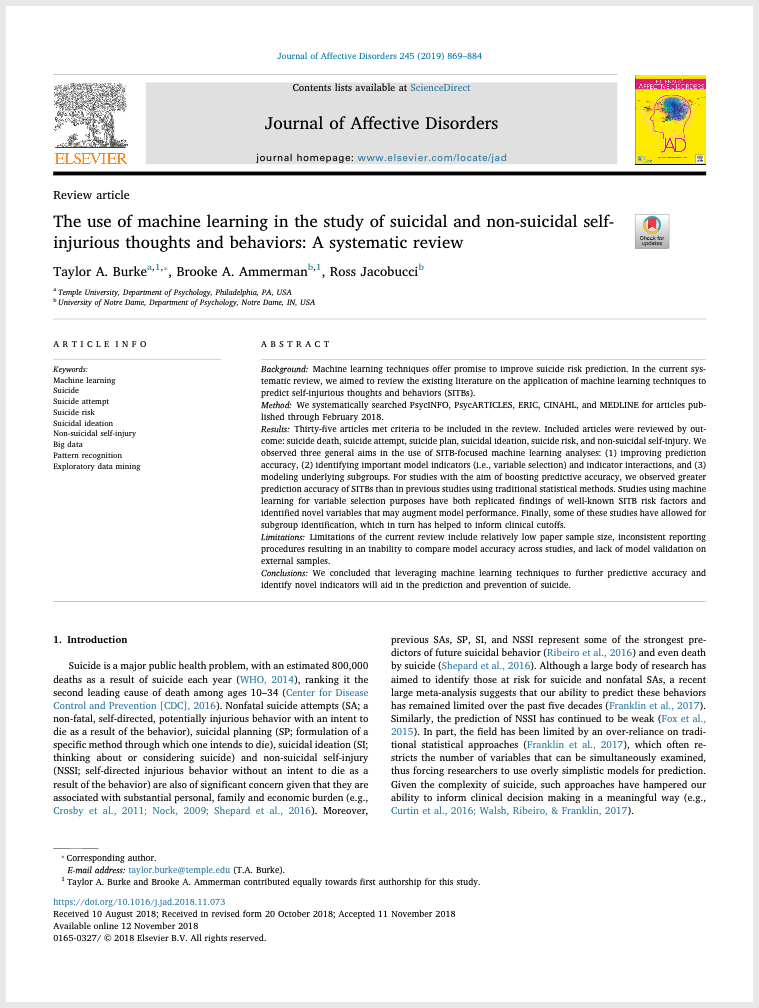
\includegraphics[scale=.4]{burke_cover.png}}
            \label{fig:burke-paper}
        \end{figure}
    }
    \frame{
        \frametitle{Consulta à Revisão Sistemática}
        \begin{figure}[h]
            \caption{Resumo de prevalência de algoritmos na revisão de Burke (2019)}
            \centerline{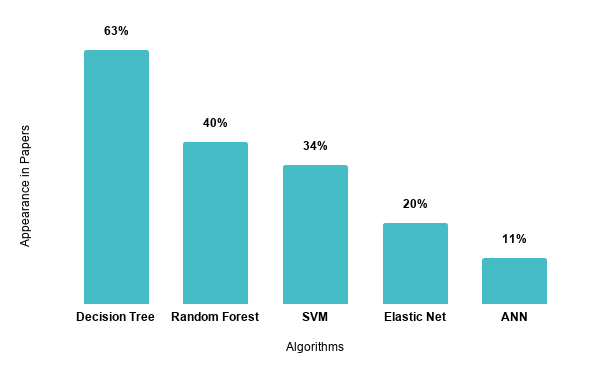
\includegraphics[scale=.45]{../fig_burke_alg_usage.png}}
            \label{fig:burke-algorithm-prevalence}
            \legend{Fonte: Autor}
        \end{figure}
    }
    \frame{
        \frametitle{Constatações da Revisão Sistemática}
        \begin{itemize}
            \item Modelos simples - interpretabilidade
            \item Tratamento de desbalanço de classes
            \item Métricas insuficientes
        \end{itemize}
    }
    \frame{
        \frametitle{Trabalhos Similares Mais Recentes}
        \begin{table}[h]
            \begin{center}
                \begin{tabular}{c|c|c|c|c|c}
                    \textit{Paper} & \textit{Algorithm} & \textit{F\textsubscript{2}-Score} & \textit{AUCROC} & \textit{Sensitivity} & \textit{Specificity} \\
                    \hline
                    \hline
                    A              & XGB                & 0.84                              & 0.86            & 0.79                 & 0.79                 \\
                    B              & ANNs/RF            & 0.71                              & 0.88            & 0.80                 & 0.79                 \\
                    C              & ANN                & 0.48                              & 0.88            & 0.81                 & 0.77                 \\
                    D              & EN                 & 0.45                              & 0.79            & 0.67                 & 0.78                 \\
                    E              & RFs                &                                   & 0.98            &                      &                      \\
                    F              & RF                 &                                   & 0.92            &                      &                      \\
                    G              & SVM                &                                   &                 & 0.77                 & 0.79                 \\
                    \hline
                \end{tabular}
            \end{center}
            \legend{
                A: JUNG et al. (2019);

                B: ROY et al. (2020);

                C: OH et al. (2020);

                D: LIBRENZA-GARCIA et al. (2020);

                E: SCHUBACH et al. (2017);

                F: GRADUS et al. (2017);

                G: BARROS et al. (2017).}
            \label{tab:related-work-comparison}
        \end{table}
    }


    \section{Metodologia}

    \begin{frame}[plain]
        \sectionpage
    \end{frame}

    \frame{
        \frametitle{Classificação de Suicidalidade}
        \begin{figure}[h]
            \caption{Modelagem de dados e classificação}
            \centerline{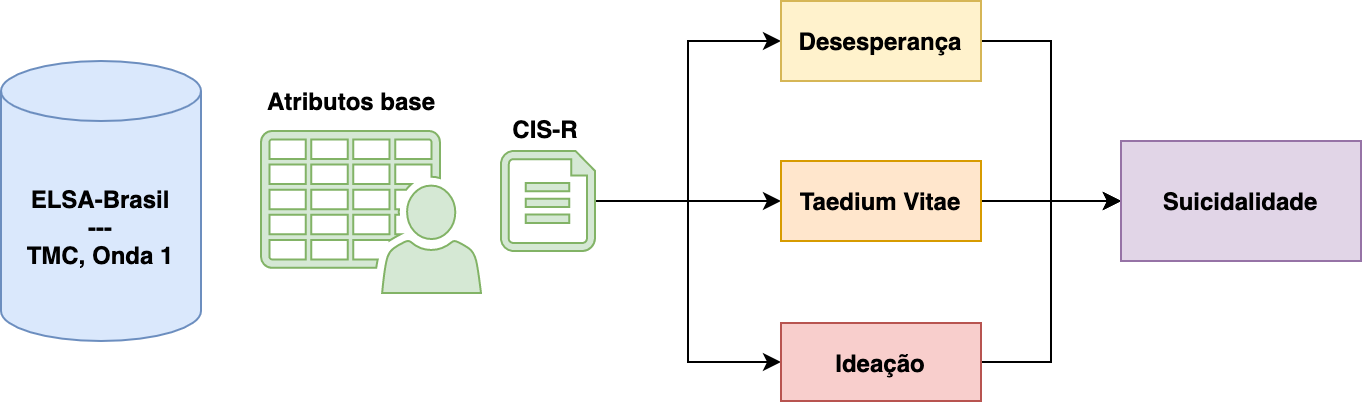
\includegraphics[scale=.22]{dados.png}}
            \label{fig:data-model}
        \end{figure}
    }
    \frame{
        \frametitle{Limpeza dos Dados - Processo}
        \begin{table}[h]
            \caption{Número de variáveis envolvidas em etapas da limpeza dos dados}
            \begin{center}
                \begin{tabular}{l|c}
                    \textit{Conjunto de Atributos}      & \textit{Tamanho do Conjunto} \\
                    \hline
                    \hline
                    Total (dados brutos)                & 2463 (100\%)                 \\
                    Removidos (vazamento de informação) & 13 (0.69\%)                  \\
                    Removidos (valores faltantes)       & 773 (31.38\%)                \\
                    Removidos (texto livre)             & 47 (1.91\%)                  \\
                    \textbf{Restante (dados limpos)}    & \textbf{1626 (66.02\%)}      \\
                    \hline
                \end{tabular}
            \end{center}
            \label{tab:dataset-cleansing}
        \end{table}


    }
    \frame{
        \frametitle{Limpeza dos Dados - Resultado}

        \begin{table}[h]
            \caption{Principais características do conjunto de dados limpo}
            \begin{center}
                \begin{tabular}{c|c}
                    \textit{Característica} & \textit{Valor} \\
                    \hline
                    \hline
                    \#Instâncias            & 4039           \\
                    \#Atributos             & 1626           \\
                    \#Positivos             & 1120 (27.73\%) \\
                    \#Negativos             & 2919 (72.27\%) \\
                    \hline
                \end{tabular}
            \end{center}
            \label{tab:final-dataset-characteristics}
        \end{table}


    }
    \frame{
        \frametitle{Pré-processamento}
        \begin{itemize}
            \item Downsampling
            \item Atribuição de valores faltantes
            \item Corte por variância quase nula
            \item Filtragem de correlações altas
            \item SMOTE - Synthetic Minority Oversampling Technique
        \end{itemize}
    }
    \frame{
        \frametitle{Algoritmos de Aprendizado}
        \begin{itemize}
            \item Elastic Nets
            \item Redes Neurais
            \item Florestas Aleatórias
        \end{itemize}
    }
    \frame{
        \frametitle{Eliminação de Atributos Recursiva (RFE)}
        \begin{figure}[h]
            \caption{Pseudocódigo do algoritmo RFE}
            \centerline{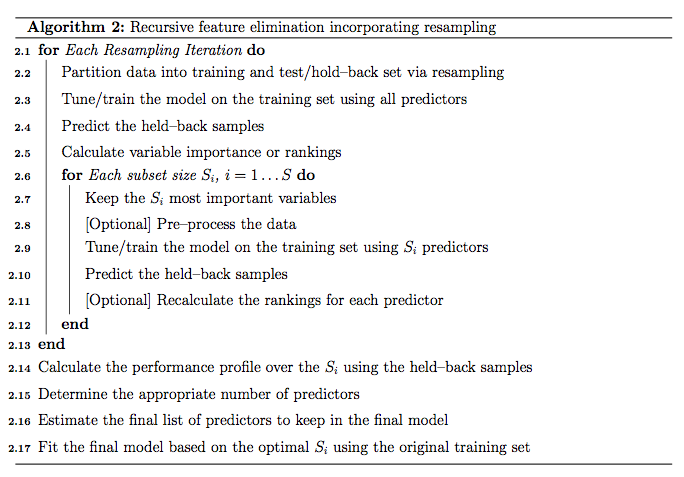
\includegraphics[scale=.35]{rfe_code.png}}
            \label{fig:rfe-code}
        \end{figure}
    }
    \frame{
        \frametitle{Métricas de Desempenho}
        \begin{itemize}
            \item Precisão (\textit{Pr}) e Recall (\textit{Re})
            \item Sensibilidade e Especificidade
            \item Área sob a curva ROC (\textit{AUCROC})
            \item F\textsubscript{2}-Score
        \end{itemize}

        \begin{equation}
            F_2 = \frac{5*TP}{5*TP+4*FN+FP}
        \end{equation}

        \begin{equation}
            F_2 = \frac{5*Pr*Re}{4*Pr+Re}
        \end{equation}
    }
    \frame{
        \frametitle{Estimativa de Desempenho}
        \begin{figure}[]
            \caption{Validação cruzada repetida e estratificada}
            \centerline{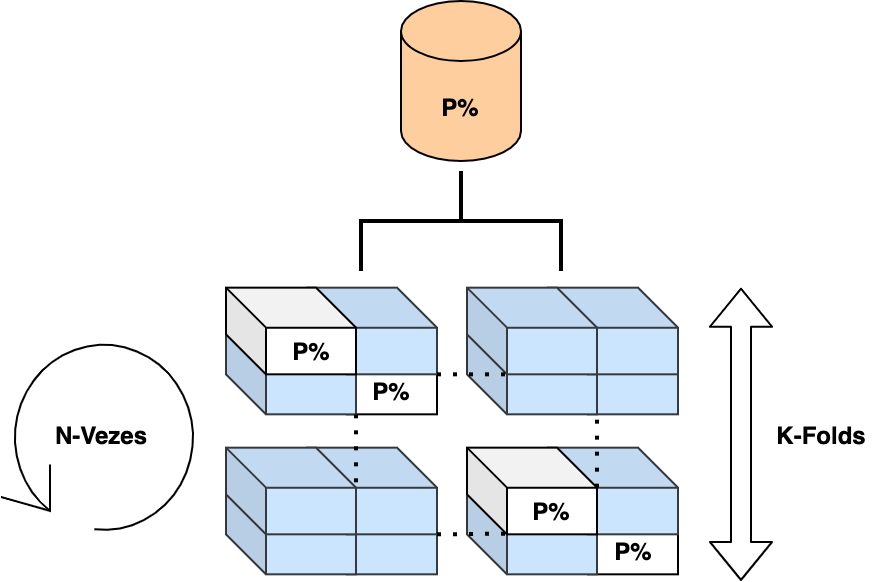
\includegraphics[scale=.3]{cross_validation.png}}
            \label{fig:cv}
        \end{figure}
    }
    \frame{
        \frametitle{Validação Cruzada Aninhada}
        \begin{figure}[]
            \centerline{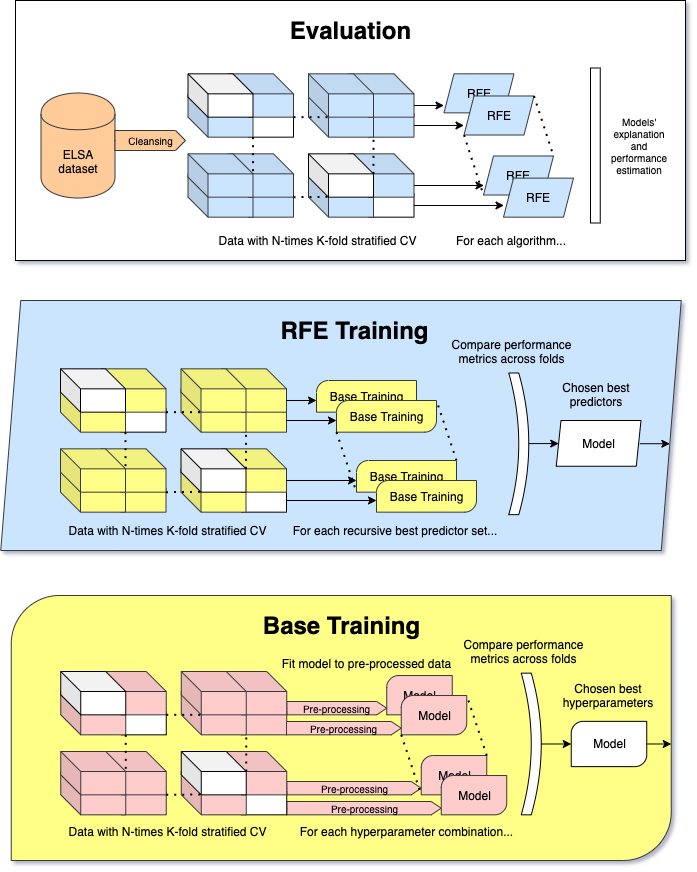
\includegraphics[scale=.25]{/home/seibel/repos/ESRP/thesis/fig_pipeline_diagram}}
            \label{fig:train-pipeline}
        \end{figure}
    }
    \frame{
        \frametitle{Modelo Ensemble}
        \begin{figure}[h]
            \centerline{\includegraphics[scale=.28]{../../notes/ensemble-diagram/ensemble.png}}
            \label{fig:ensemble}
        \end{figure}
    }


    \section{Experimentos}
    \begin{frame}[plain]
        \sectionpage
    \end{frame}

    \frame{
        \frametitle{Metaparâmetros - Pipeline}
        \begin{table}[h]
            \begin{center}
                \begin{tabular}{l|c}
                    \textit{Parameter}            & \textit{Value}                    \\
                    \hline
                    \hline
                    CV Avaliação - K (folds)      & 10                                \\
                    CV Avaliação - N (vezes)      & 3                                 \\
                    CV Treino RFE - K (folds)     & 5                                 \\
                    CV Treino RFE - N (vezes)     & 2                                 \\
                    CV Treino Base - K (folds)    & 5                                 \\
                    CV Treino Base - N (vezes)    & 2                                 \\
                    Downsampling - Taxa positivos & 33.3\%                            \\
                    SMOTE - Taxa positivos        & 50\%                              \\
                    RFE - Número de atributos     & (2^k)$^{\text{k=9}}_{\text{k=3}}$ \\
                    \hline
                \end{tabular}
            \end{center}
            \label{tab:pipeline-parameters-experiments}
        \end{table}
    }
    \frame{
        \frametitle{Hiperparâmetros - Modelos}
        \begin{itemize}
            \item Busca em grade
        \end{itemize}
        \begin{table}[h]
            \begin{center}
                \begin{tabular}{l|c}
                    \textit{Parâmetro}              & \textit{Valores}                       \\
                    \hline
                    \hline
                    Elastic Net - Alpha             & 0.1 , 0.325 , 0.550 , 0.775 , 1        \\
                    Elastic Net - Lambda            & 2e-4 , 9.2e-4 , 4.3e-3 , 2e-2 , 9.2e-2 \\
                    Rede Neural - Camada 1          & 1 , 2 , 3 , 4 , 5                      \\
                    Rede Neural - Camada 2          & 0 , 1 , 2 , 3 , 4                      \\
                    Floresta Aleatória - Atributos  & 2, 17, 33, 48, 64                      \\
                    Floresta Aleatória - Node-split & \textit{gini}, \textit{extratrees}     \\
                    Ensemble - Pesos dos modelos    & 1/3                                    \\
                    \hline
                \end{tabular}
            \end{center}
            \label{tab:hyperparameters}
        \end{table}
    }

    \frame{
        \frametitle{Implementação}
        Linguagem \textit{R}\linebreak

        Pacotes principais:
        \begin{itemize}
            \item \textit{caret}
            \item \textit{recipes}
            \item \textit{dplyr}
            \item \textit{purrr}
            \item \textit{ggplot2}
        \end{itemize}
    }


    \section{Resultados}
    \begin{frame}[plain]
        \sectionpage
    \end{frame}

    \frame{
        \frametitle{Resumo Estimativa de Desempenho}
        \begin{table}[h]
            \caption{Médias e desvios padrão de estimativas de desempenho}
            \begin{center}
                \begin{tabular}{c|c|c|c|c|c|c|c|c}
                    \textit{Algoritmo} & \textit{F\textsubscript{2}-Score} & \textit{AUCROC}    & \textit{Sens.}     & \textit{Espe.}     \\
                    \hline
                    \hline
                    Ensemble           & 0.69 \textpm\ 0.03                & 0.81 \textpm\ 0.02 & 0.78 \textpm\ 0.05 & 0.67 \textpm\ 0.05 \\
                    R. Neurais         & 0.69 \textpm\ 0.04                & 0.76 \textpm\ 0.08 & 0.81 \textpm\ 0.09 & 0.59 \textpm\ 0.17 \\
                    Elastic N.         & 0.66 \textpm\ 0.07                & 0.77 \textpm\ 0.04 & 0.75 \textpm\ 0.11 & 0.66 \textpm\ 0.09 \\
                    Florestas A.       & 0.61 \textpm\ 0.04                & 0.81 \textpm\ 0.02 & 0.63 \textpm\ 0.05 & 0.79 \textpm\ 0.03 \\
                    \hline
                \end{tabular}
            \end{center}
            \label{tab:final-performance-estimates}
        \end{table}
    }
    \frame{
        \frametitle{Desempenho por F2-Score}
        \begin{figure}[H]
            \centerline{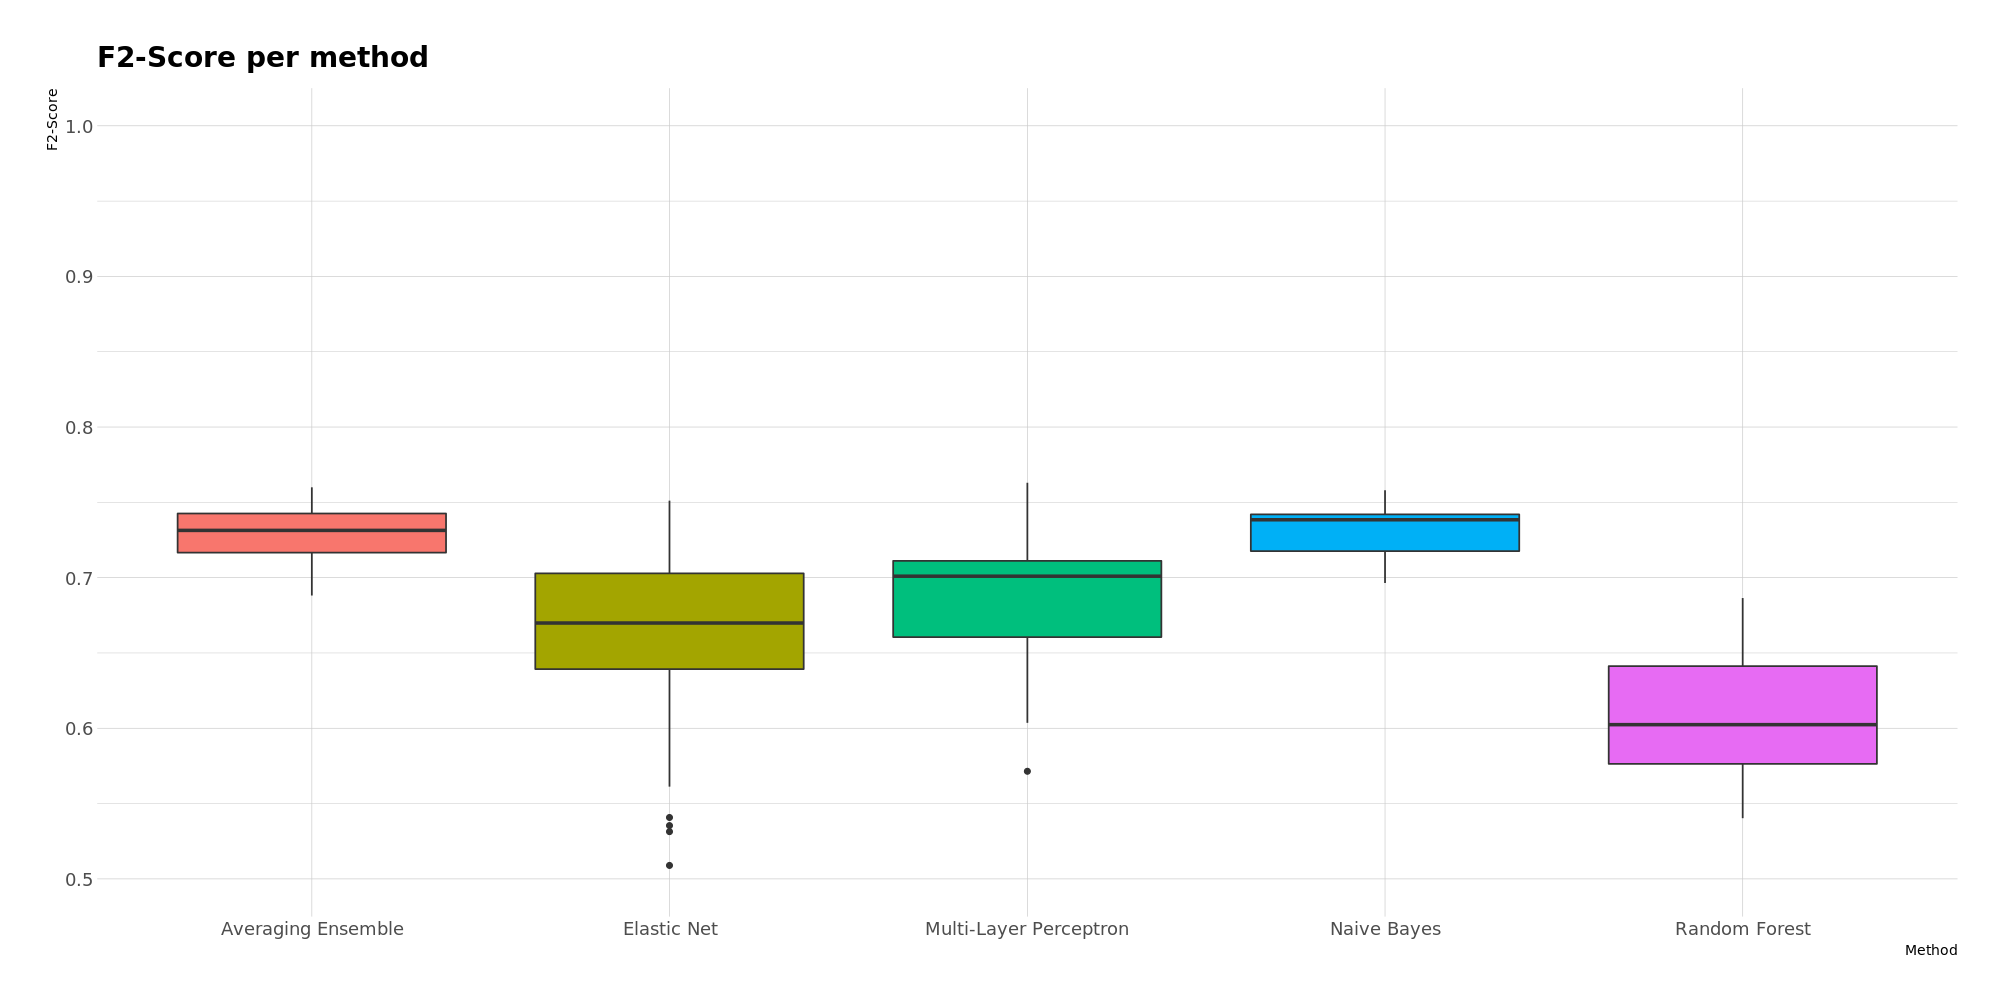
\includegraphics[scale=.16]{../../reports/results/models_and_evals/summary/box_plot_f2.png}}
            \legend{Source: Author}
        \end{figure}
    }
    \frame{
        \frametitle{Desempenho por AUCROC}
        \begin{figure}[H]
            \centerline{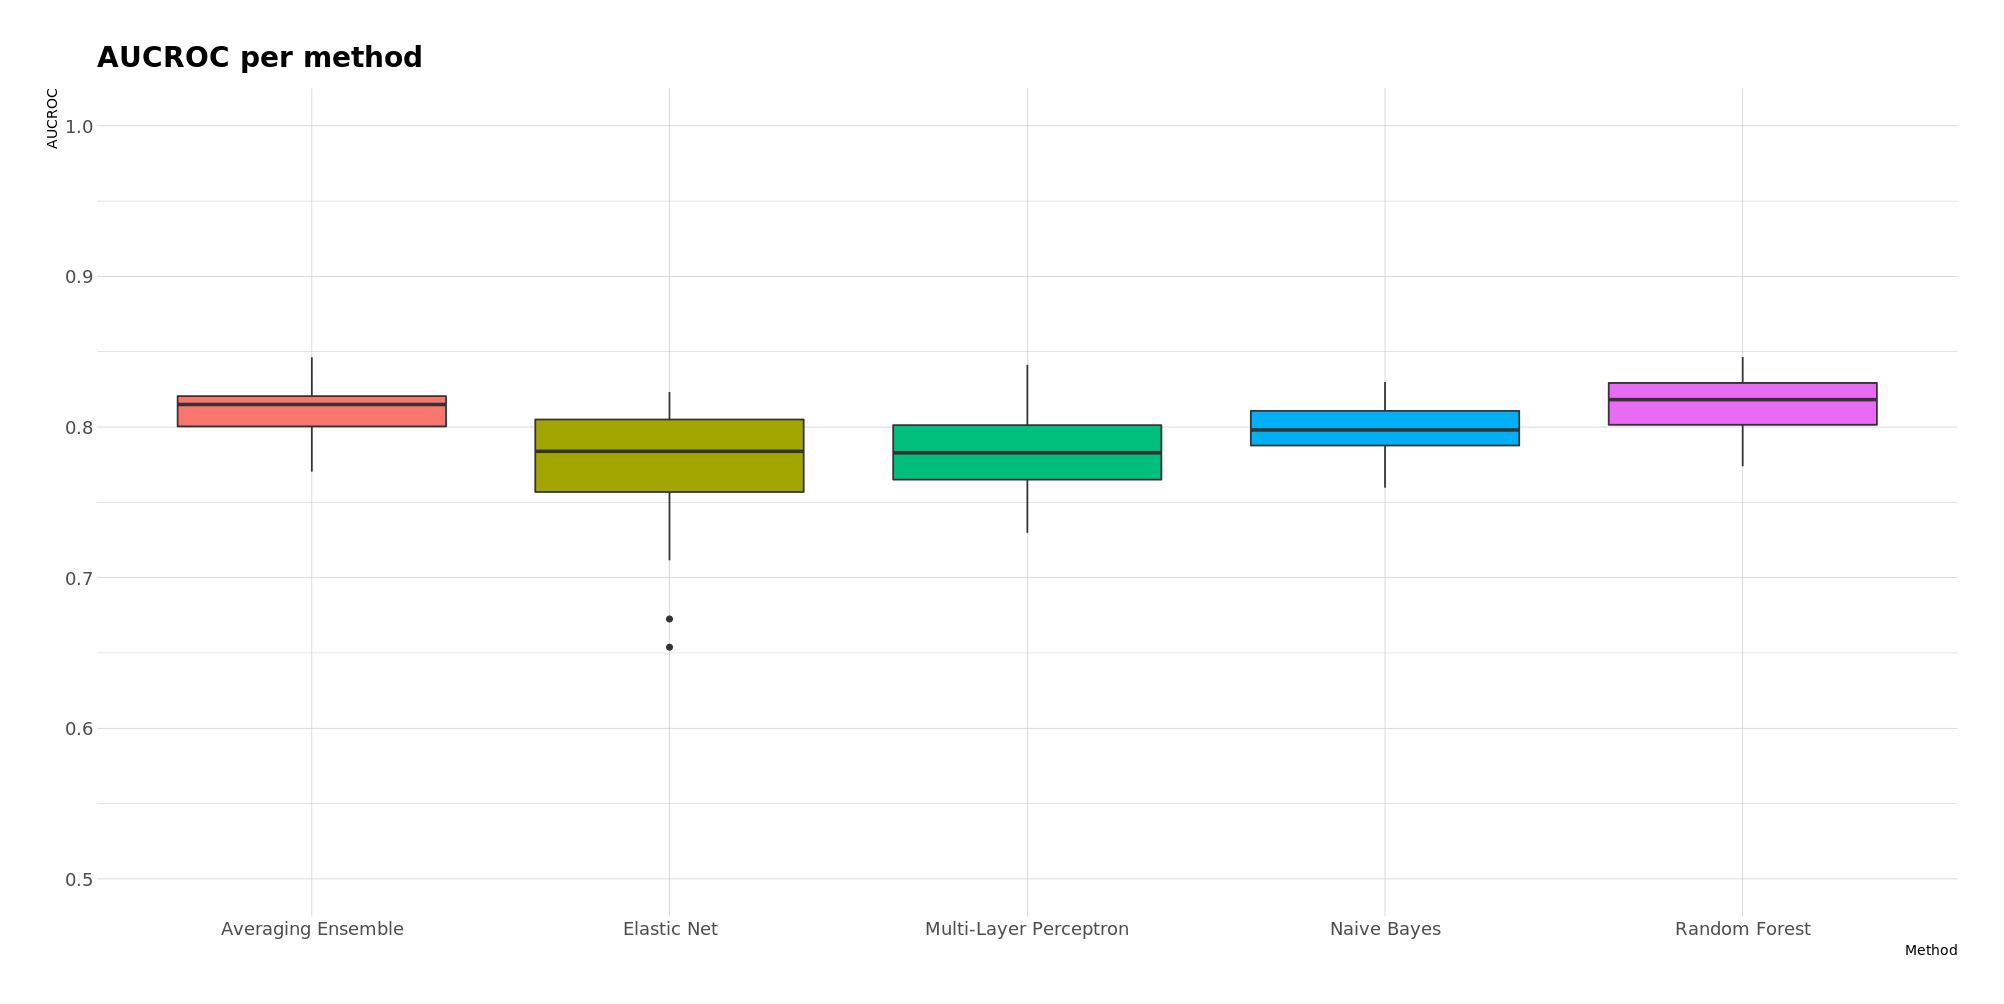
\includegraphics[scale=.16]{../../reports/results/models_and_evals/summary/box_plot_aucroc.png}}
            \legend{Source: Author}
        \end{figure}
    }
    \frame{
        \frametitle{Desempenho por Sensibilidade}
        \begin{figure}[H]
            \centerline{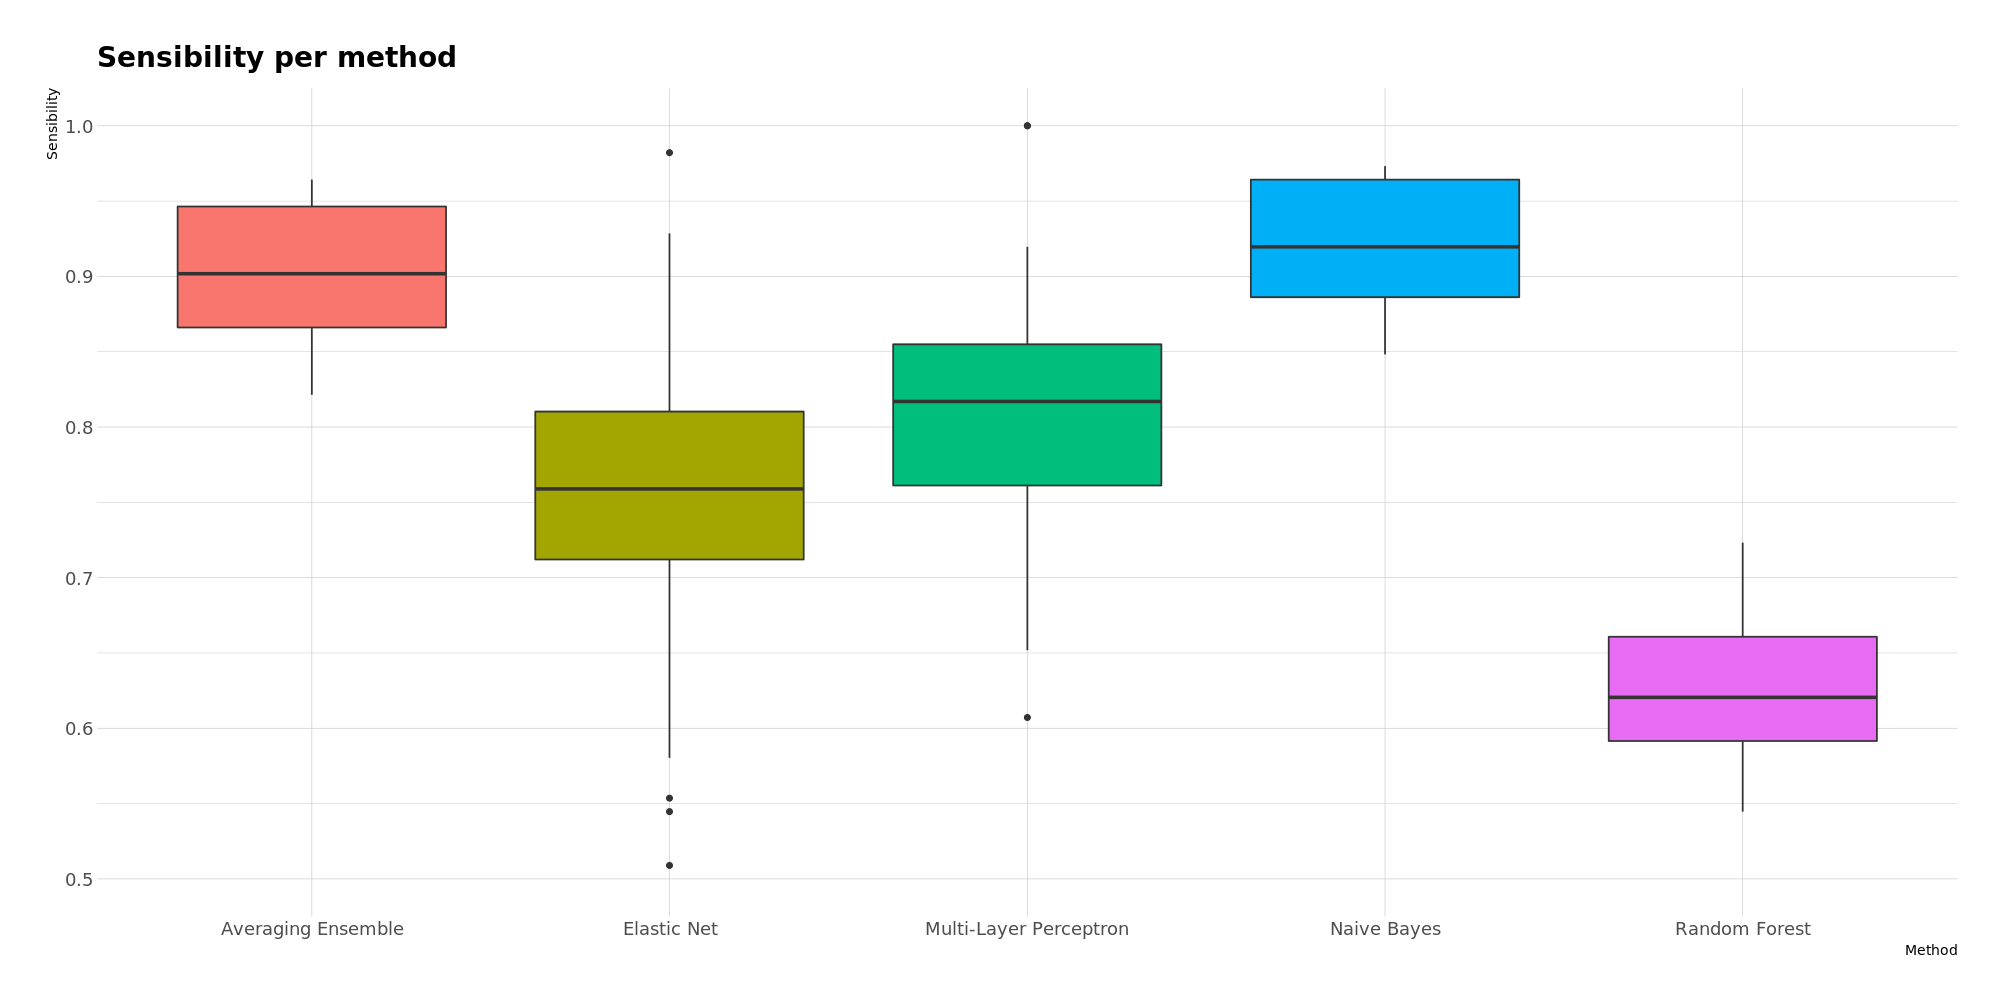
\includegraphics[scale=.16]{../../reports/results/models_and_evals/summary/box_plot_sens.png}}
            \label{fig:boxplot-sens}
        \end{figure}
    }
    \frame{
        \frametitle{Desempenho por Especificidade}
        \begin{figure}[H]
            \centerline{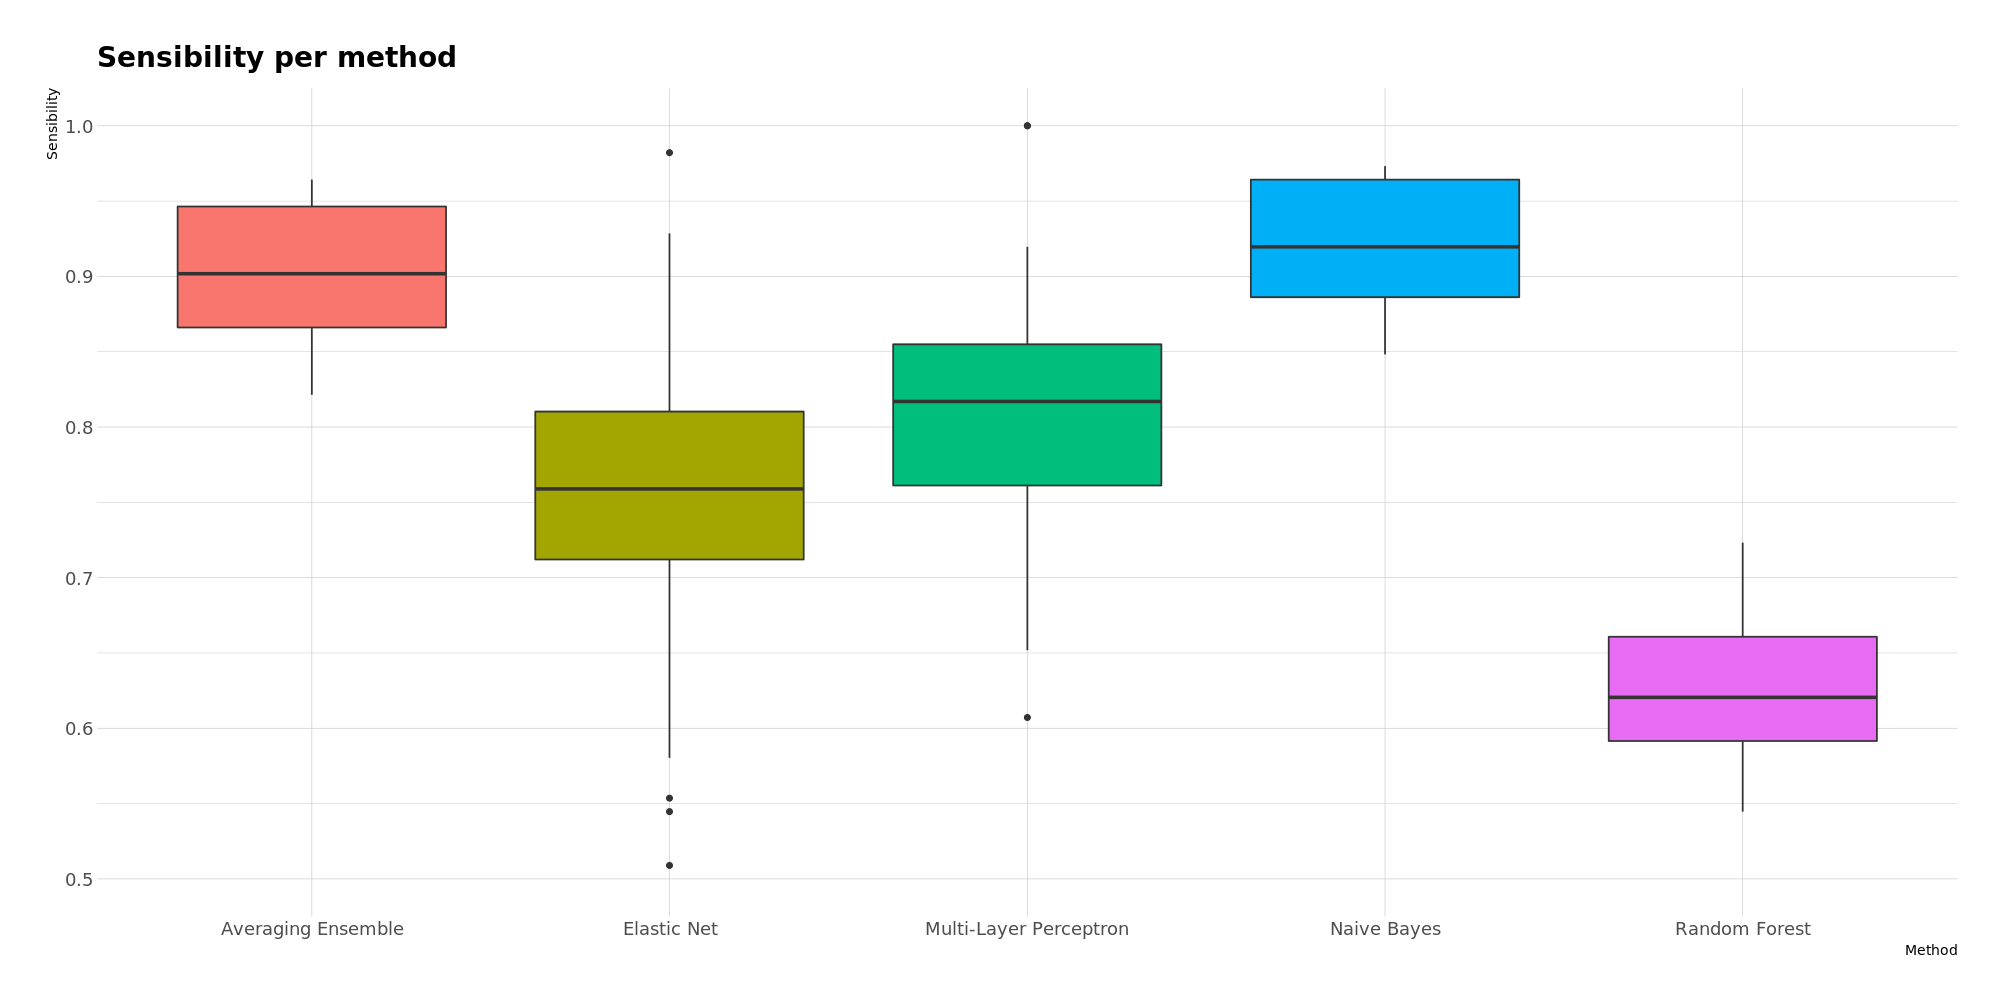
\includegraphics[scale=.16]{../../reports/results/models_and_evals/summary/box_plot_spec.png}}
            \label{fig:boxplot-spec}
        \end{figure}
    }
    \frame{
        \frametitle{Seleção de Atributos - Elastic Nets}
        \begin{figure}[H]
            \centerline{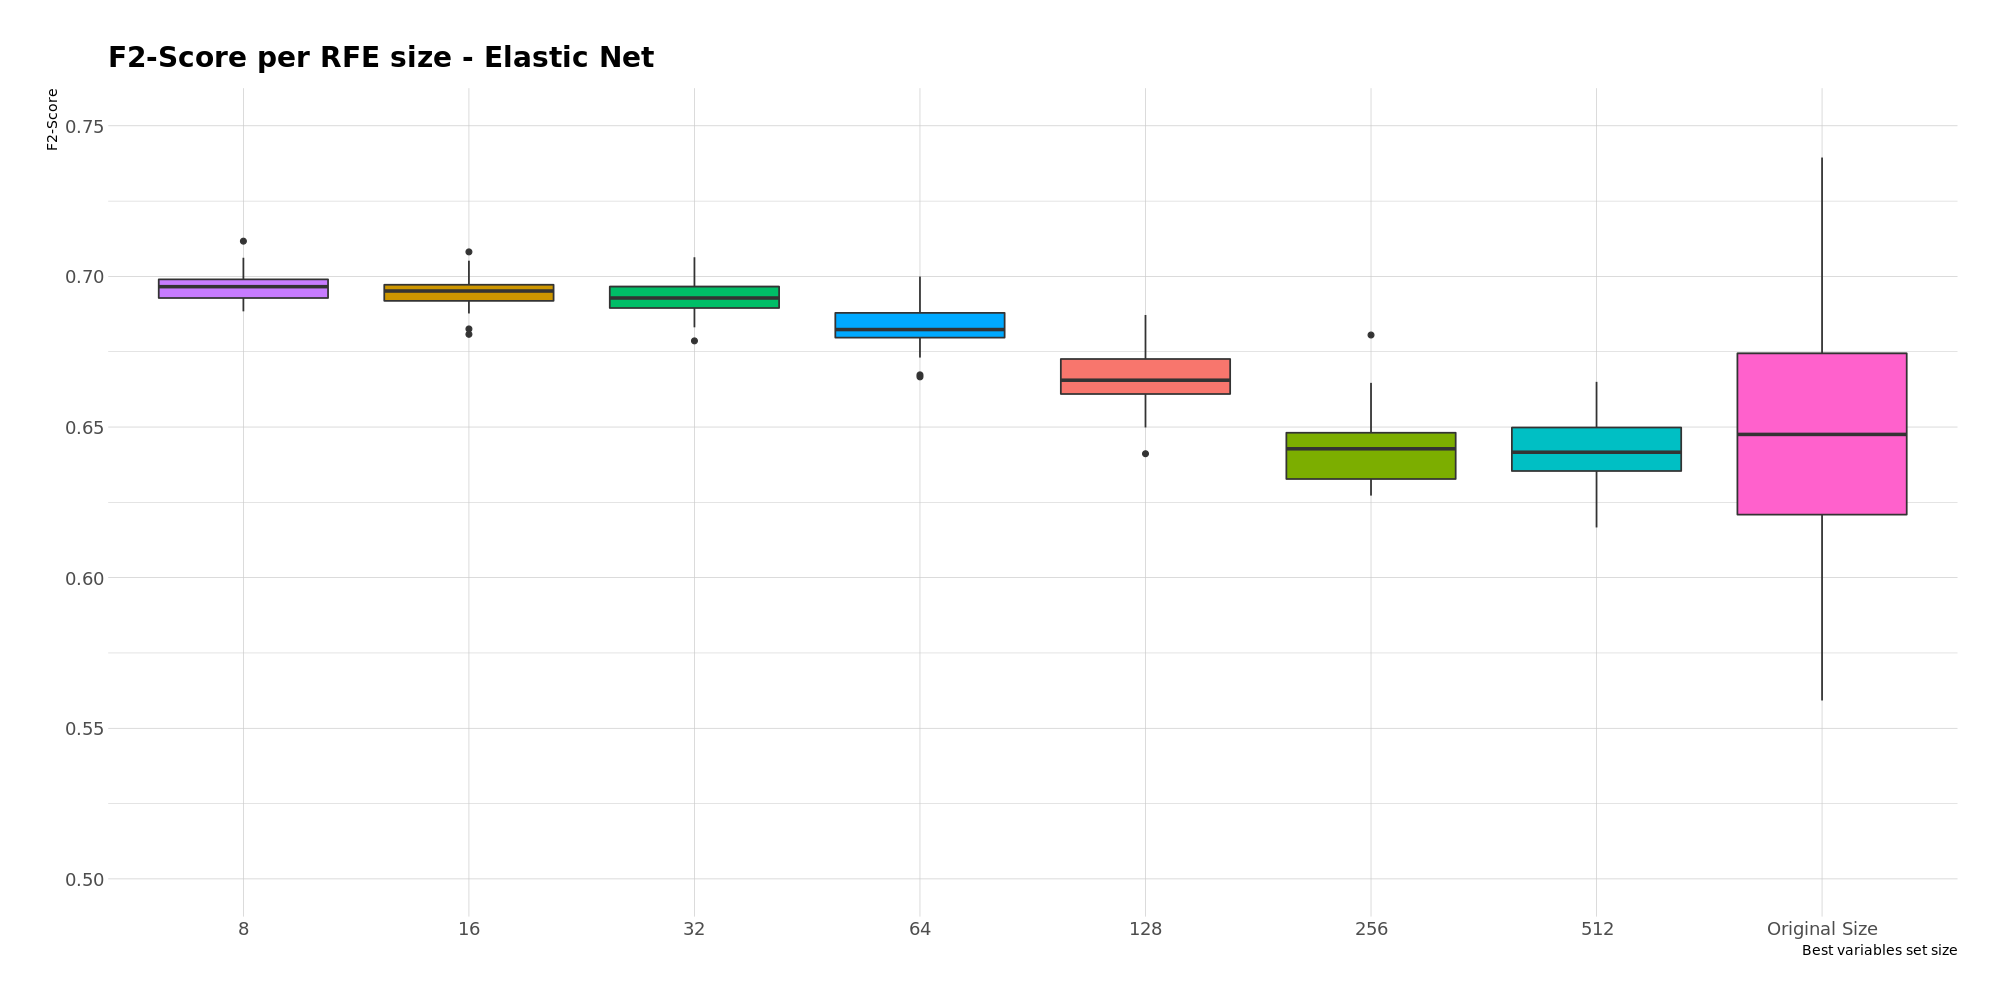
\includegraphics[scale=.16]{../../reports/results/models_and_evals/summary/rfe_glmnet.png}}
            \label{fig:rfe-glmnet}
        \end{figure}
    }
    \frame{
        \frametitle{Seleção de Atributos - Redes Neurais}
        \begin{figure}[H]
            \centerline{\includegraphics[scale=.16]{../../reports/results/models_and_evals/summary/rfe_mlpML.png}}
            \label{fig:rfe-mlp}
        \end{figure}
    }
    \frame{
        \frametitle{Seleção de Atributos - Florestas Aleatórias}
        \begin{figure}[H]
            \centerline{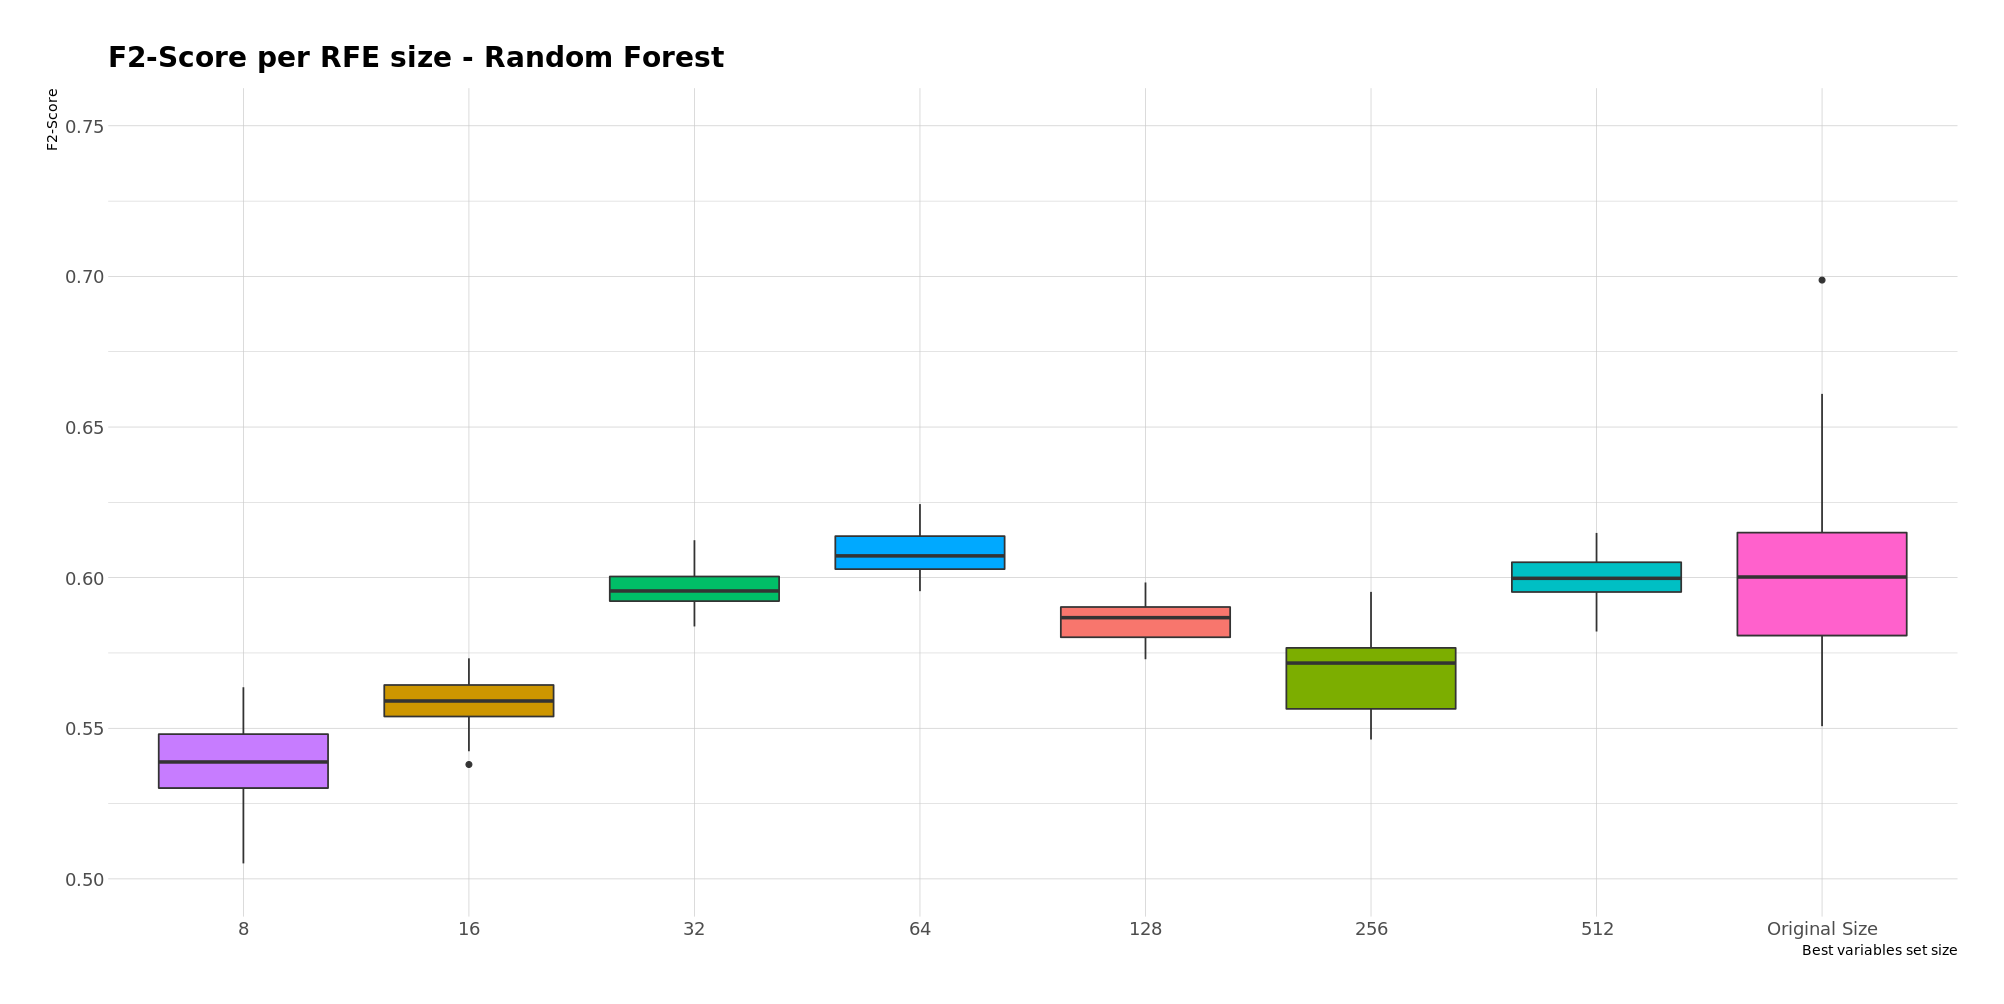
\includegraphics[scale=.16]{../../reports/results/models_and_evals/summary/rfe_ranger.png}}
            \label{fig:rfe-ranger}
        \end{figure}
    }
%    \frame{
%    \frametitle{Hiperparâmetros mais Frequentes}
%    \begin{table}[h]
%        \begin{center}
%            \begin{tabular}{l|c}
%                \textit{Parameter}              & \textit{Value}      \\
%                \hline
%                \hline
%                Elastic Net - Alpha             & 0.1                 \\
%                Elastic Net - Lambda            & 0.09                \\
%                Rede Neural - Camada 1          & 1                   \\
%                Rede Neural - Camada 2          & 1                   \\
%                Floresta Aleatória - Atributos  & 2                   \\
%                Floresta Aleatória - Node-split & \textit{extratrees} \\
%                \hline
%            \end{tabular}
%        \end{center}
%        \label{tab:most-frequent-hyperparams}
%    \end{table}
%    }
    \frame{
        \frametitle{Mapa de Atributos - Elastic Nets}
        \begin{figure}[H]
            \centerline{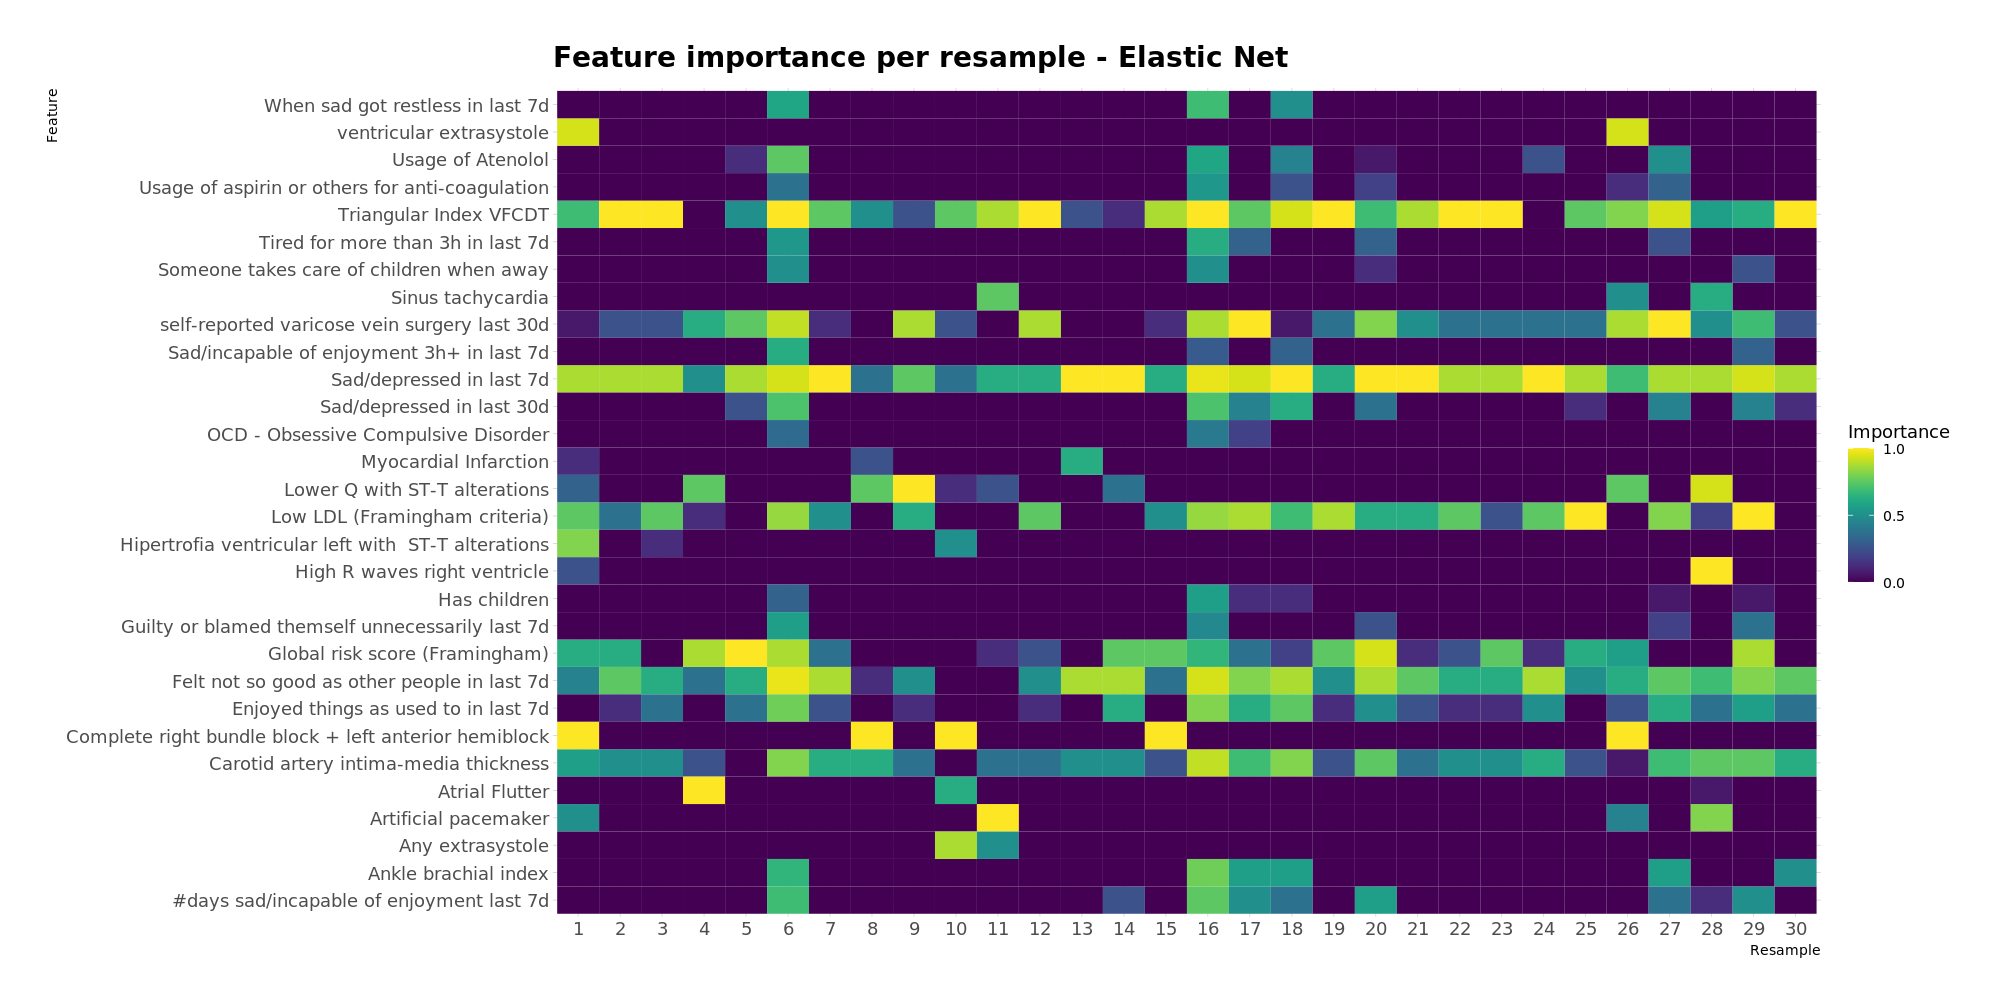
\includegraphics[scale=.16]{../../reports/results/models_and_evals/summary/var_imp_resample_glmnet.png}}
            \label{fig:heatmap-glmnet}
        \end{figure}
    }
    \frame{
        \frametitle{Mapa de Atributos - Redes Neurais}
        \begin{figure}[H]
            \centerline{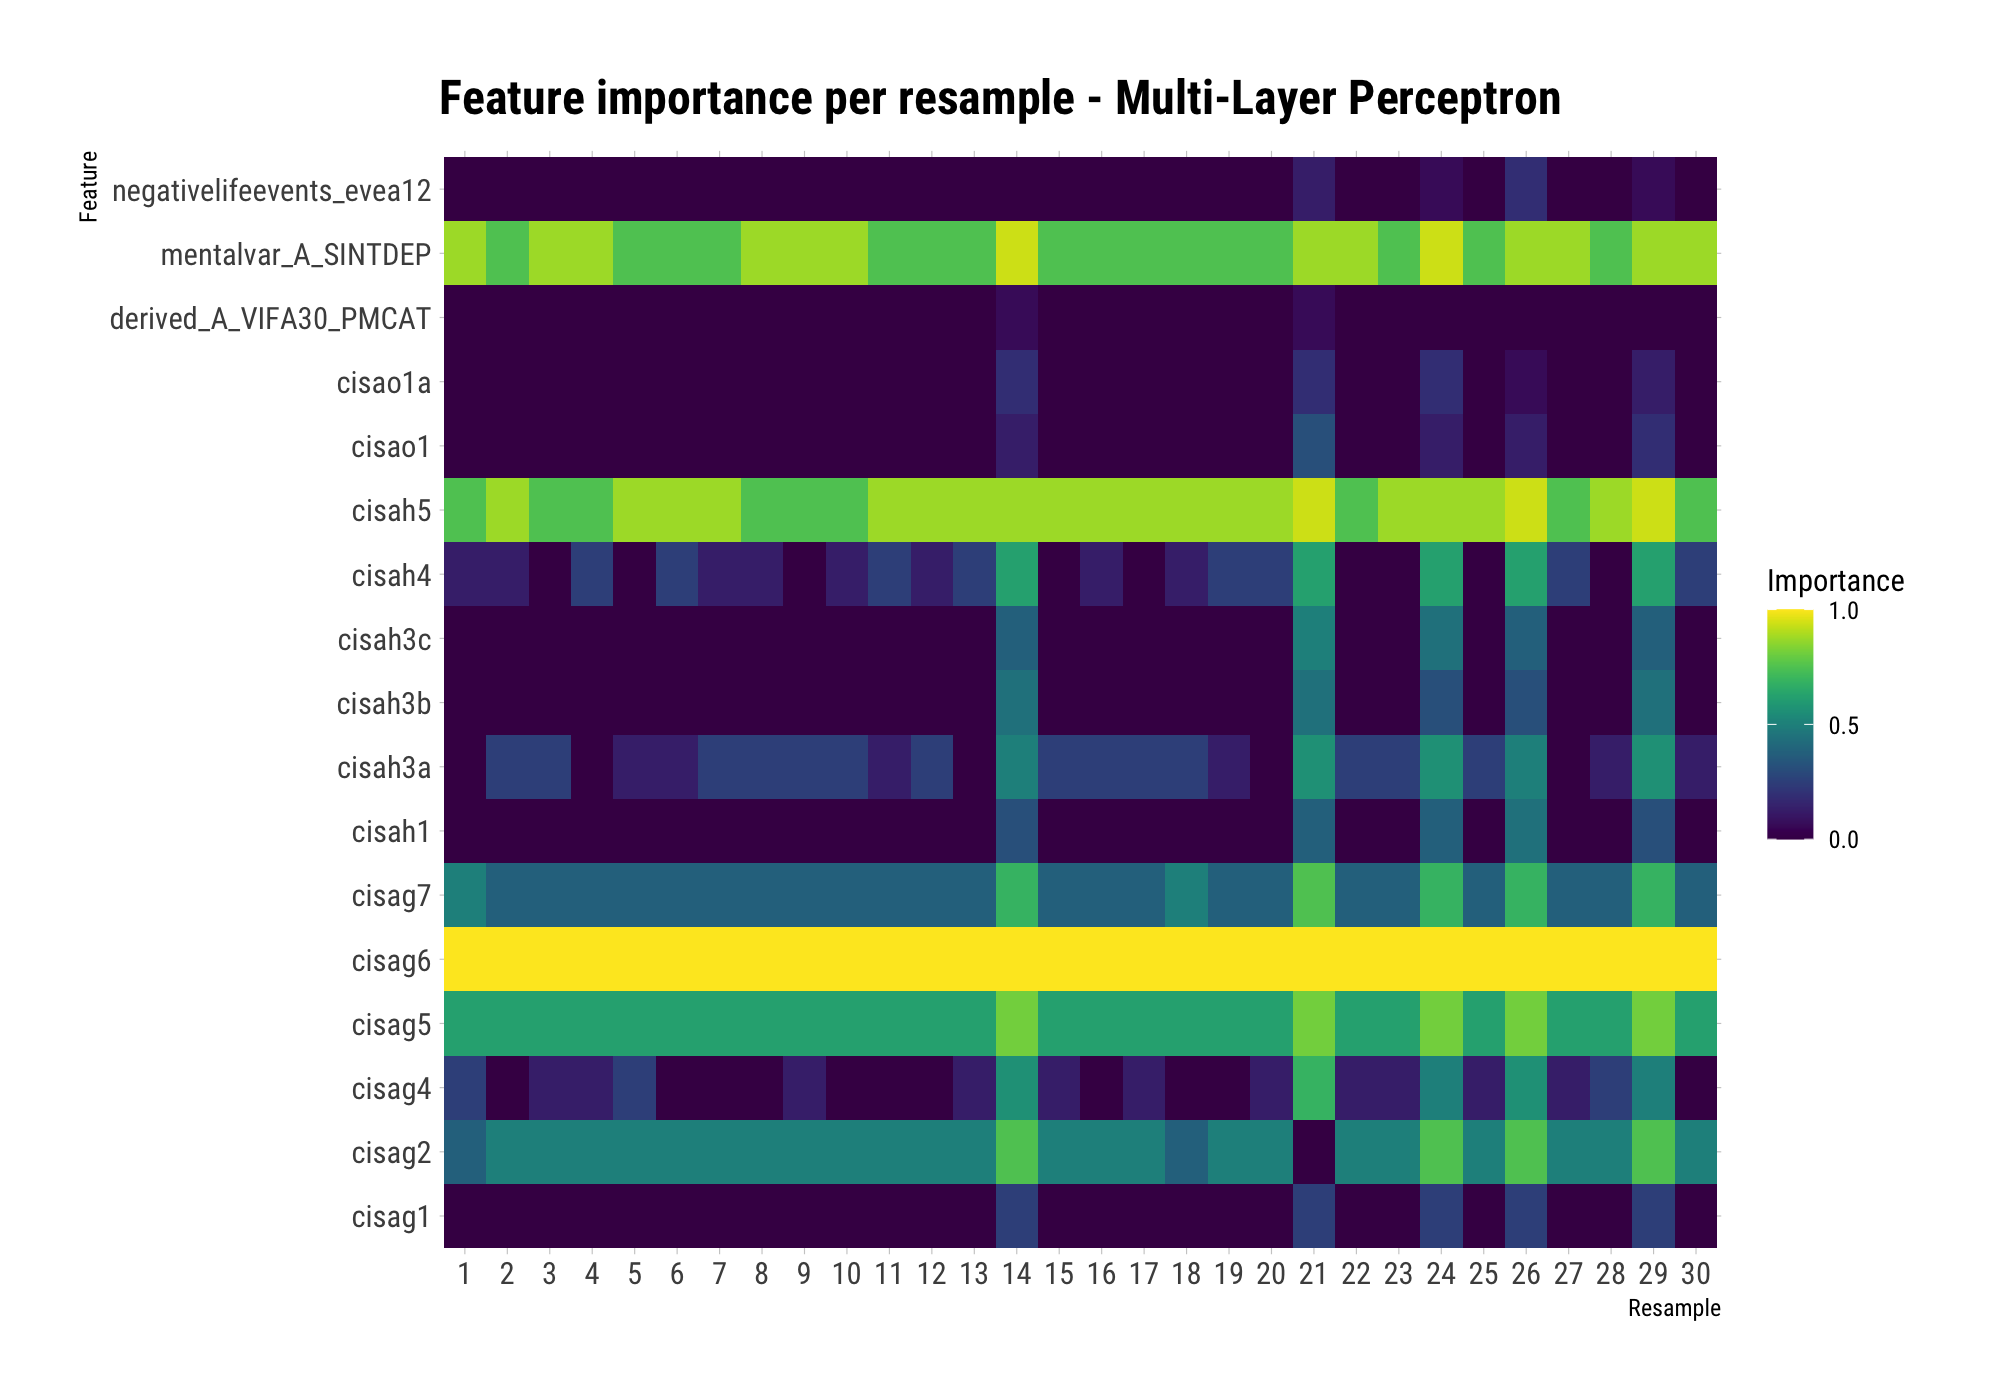
\includegraphics[scale=.16]{../../reports/results/models_and_evals/summary/var_imp_resample_mlpML.png}}
            \label{fig:heatmap-mlp}
        \end{figure}
    }
    \frame{
        \frametitle{Mapa de Atributos - Florestas Aleatórias}
        \begin{figure}[H]
            \centerline{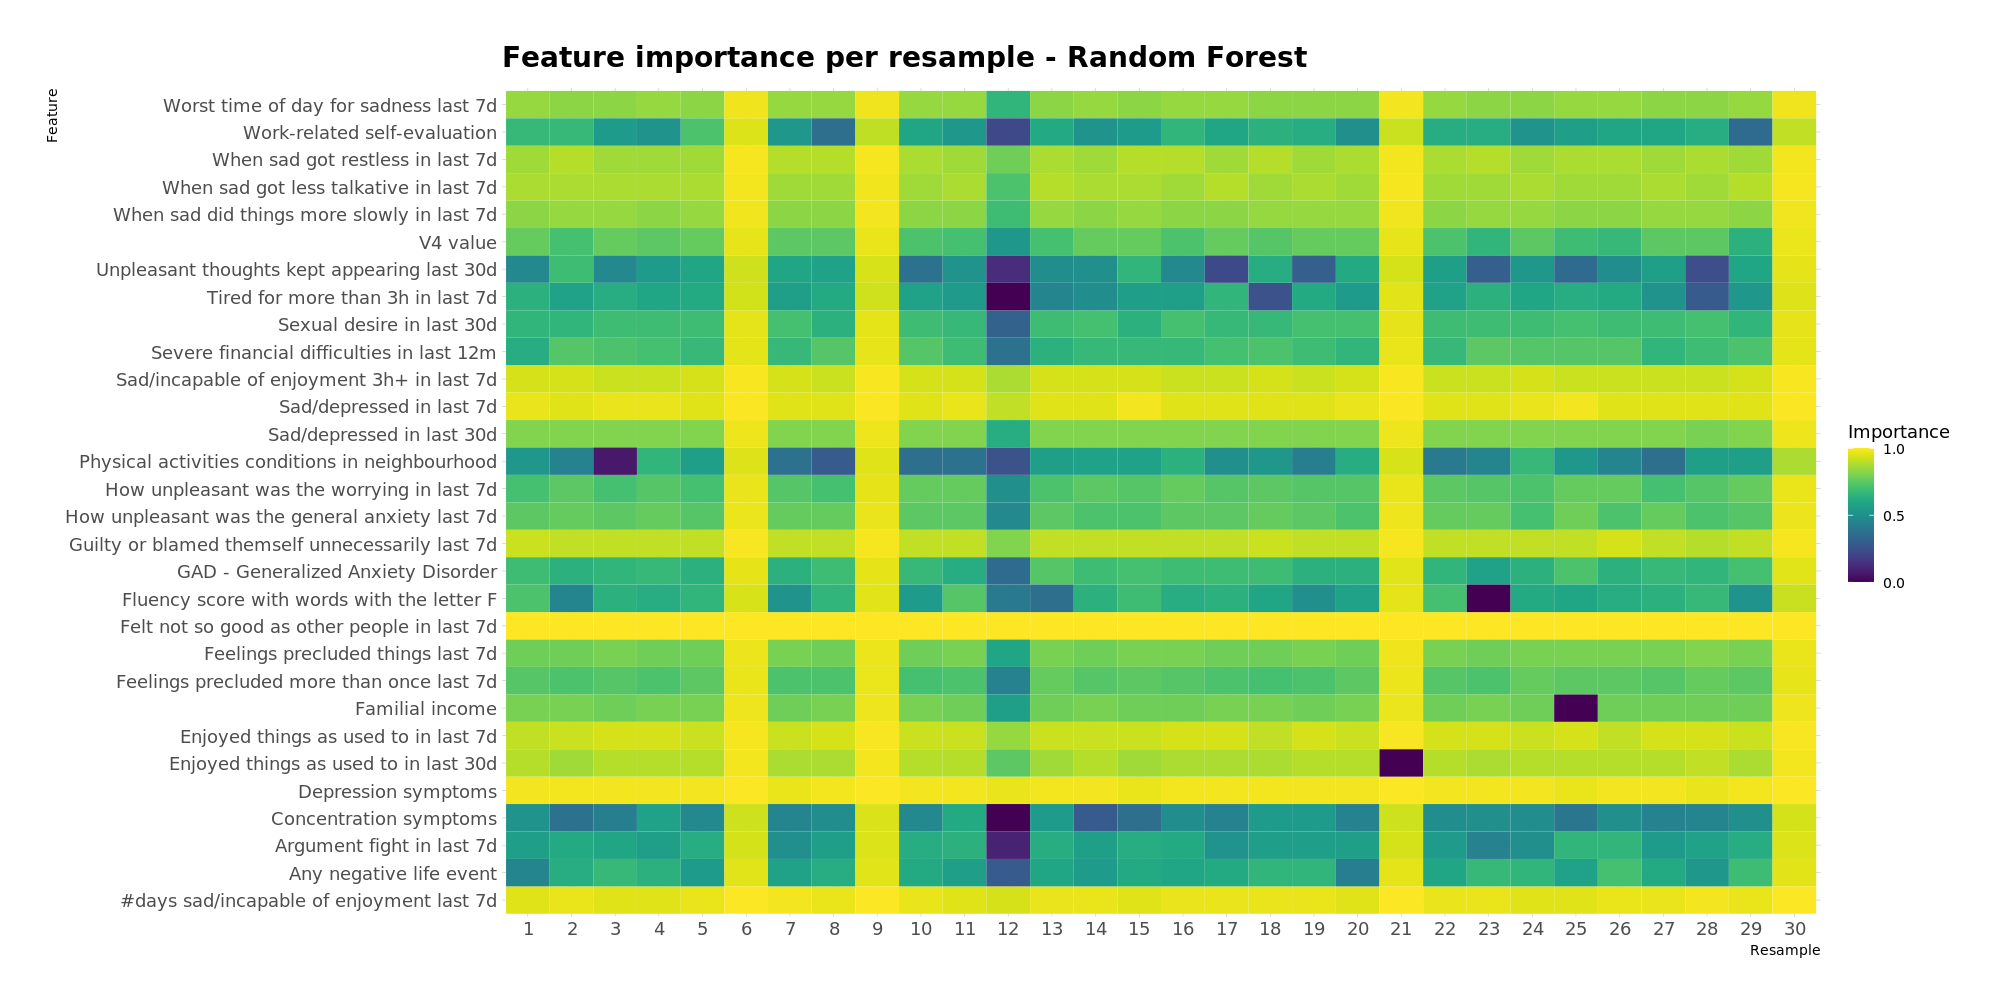
\includegraphics[scale=.16]{../../reports/results/models_and_evals/summary/var_imp_resample_ranger.png}}
            \label{fig:heatmap-ranger}
        \end{figure}
    }
    \frame{
        \frametitle{Mapa de Atributos - Ensemble}
        \begin{figure}[H]
            \centerline{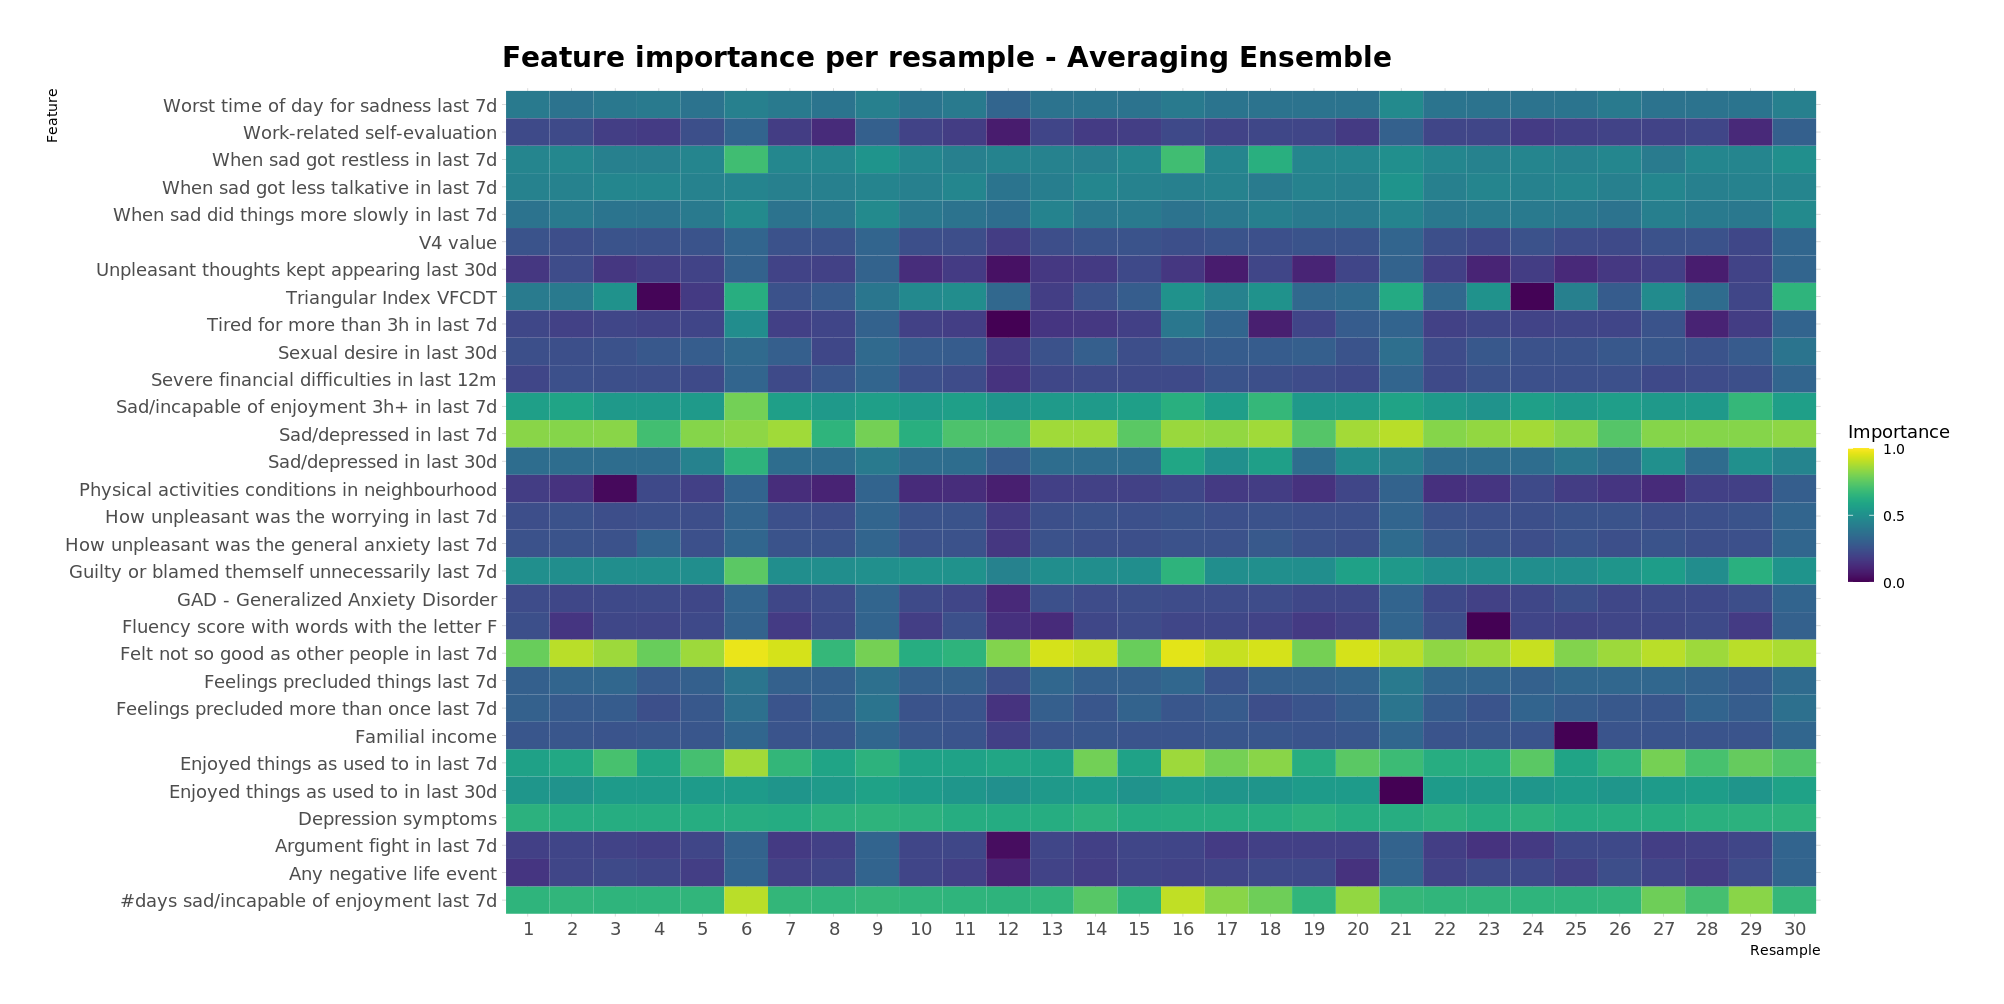
\includegraphics[scale=.16]{../../reports/results/models_and_evals/summary/var_imp_resample_aggregation.png}}
            \label{fig:heatmap-ensemble}
        \end{figure}
    }
    \frame{
        \frametitle{Rank de Atributos - Elastic Nets}
        \begin{figure}[H]
            \centerline{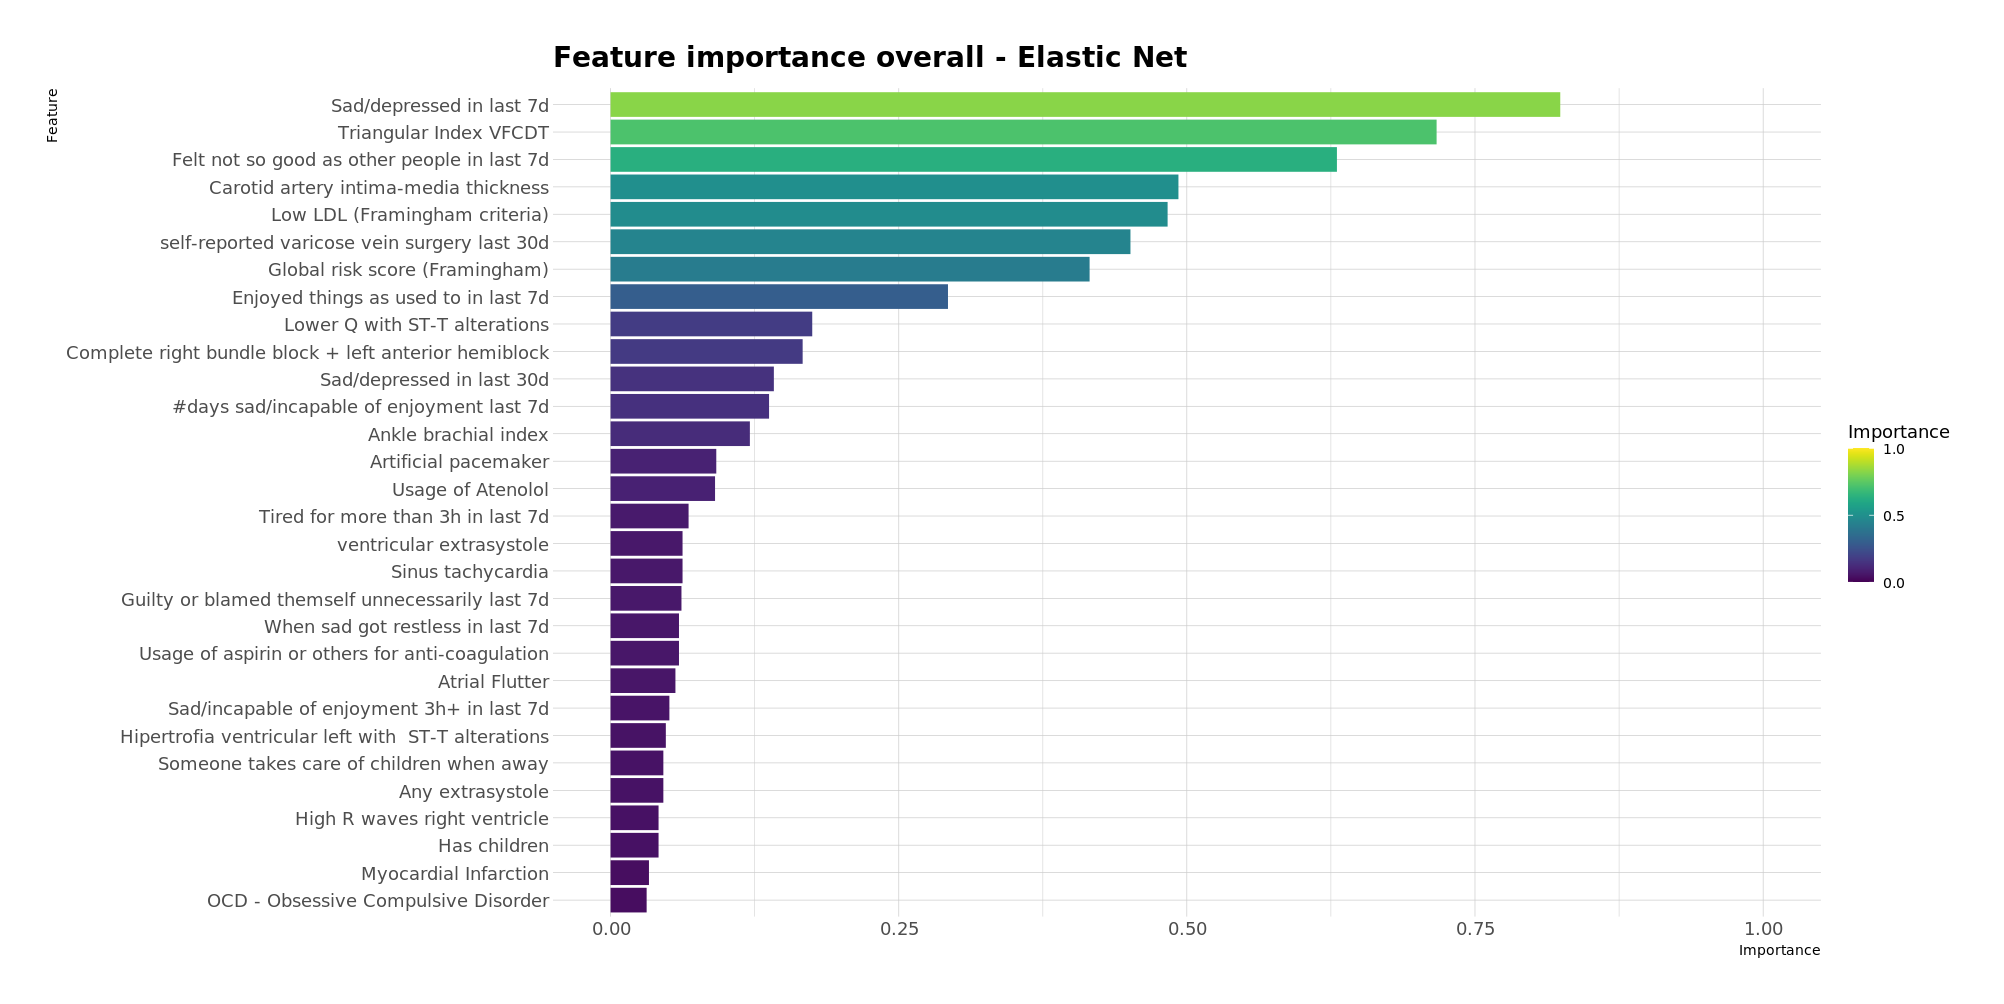
\includegraphics[scale=.16]{../../reports/results/models_and_evals/summary/var_imp_glmnet.png}}
            \label{fig:rank-glmnet}
        \end{figure}
    }
    \frame{
        \frametitle{Rank de Atributos - Redes Neurais}
        \begin{figure}[H]
            \centerline{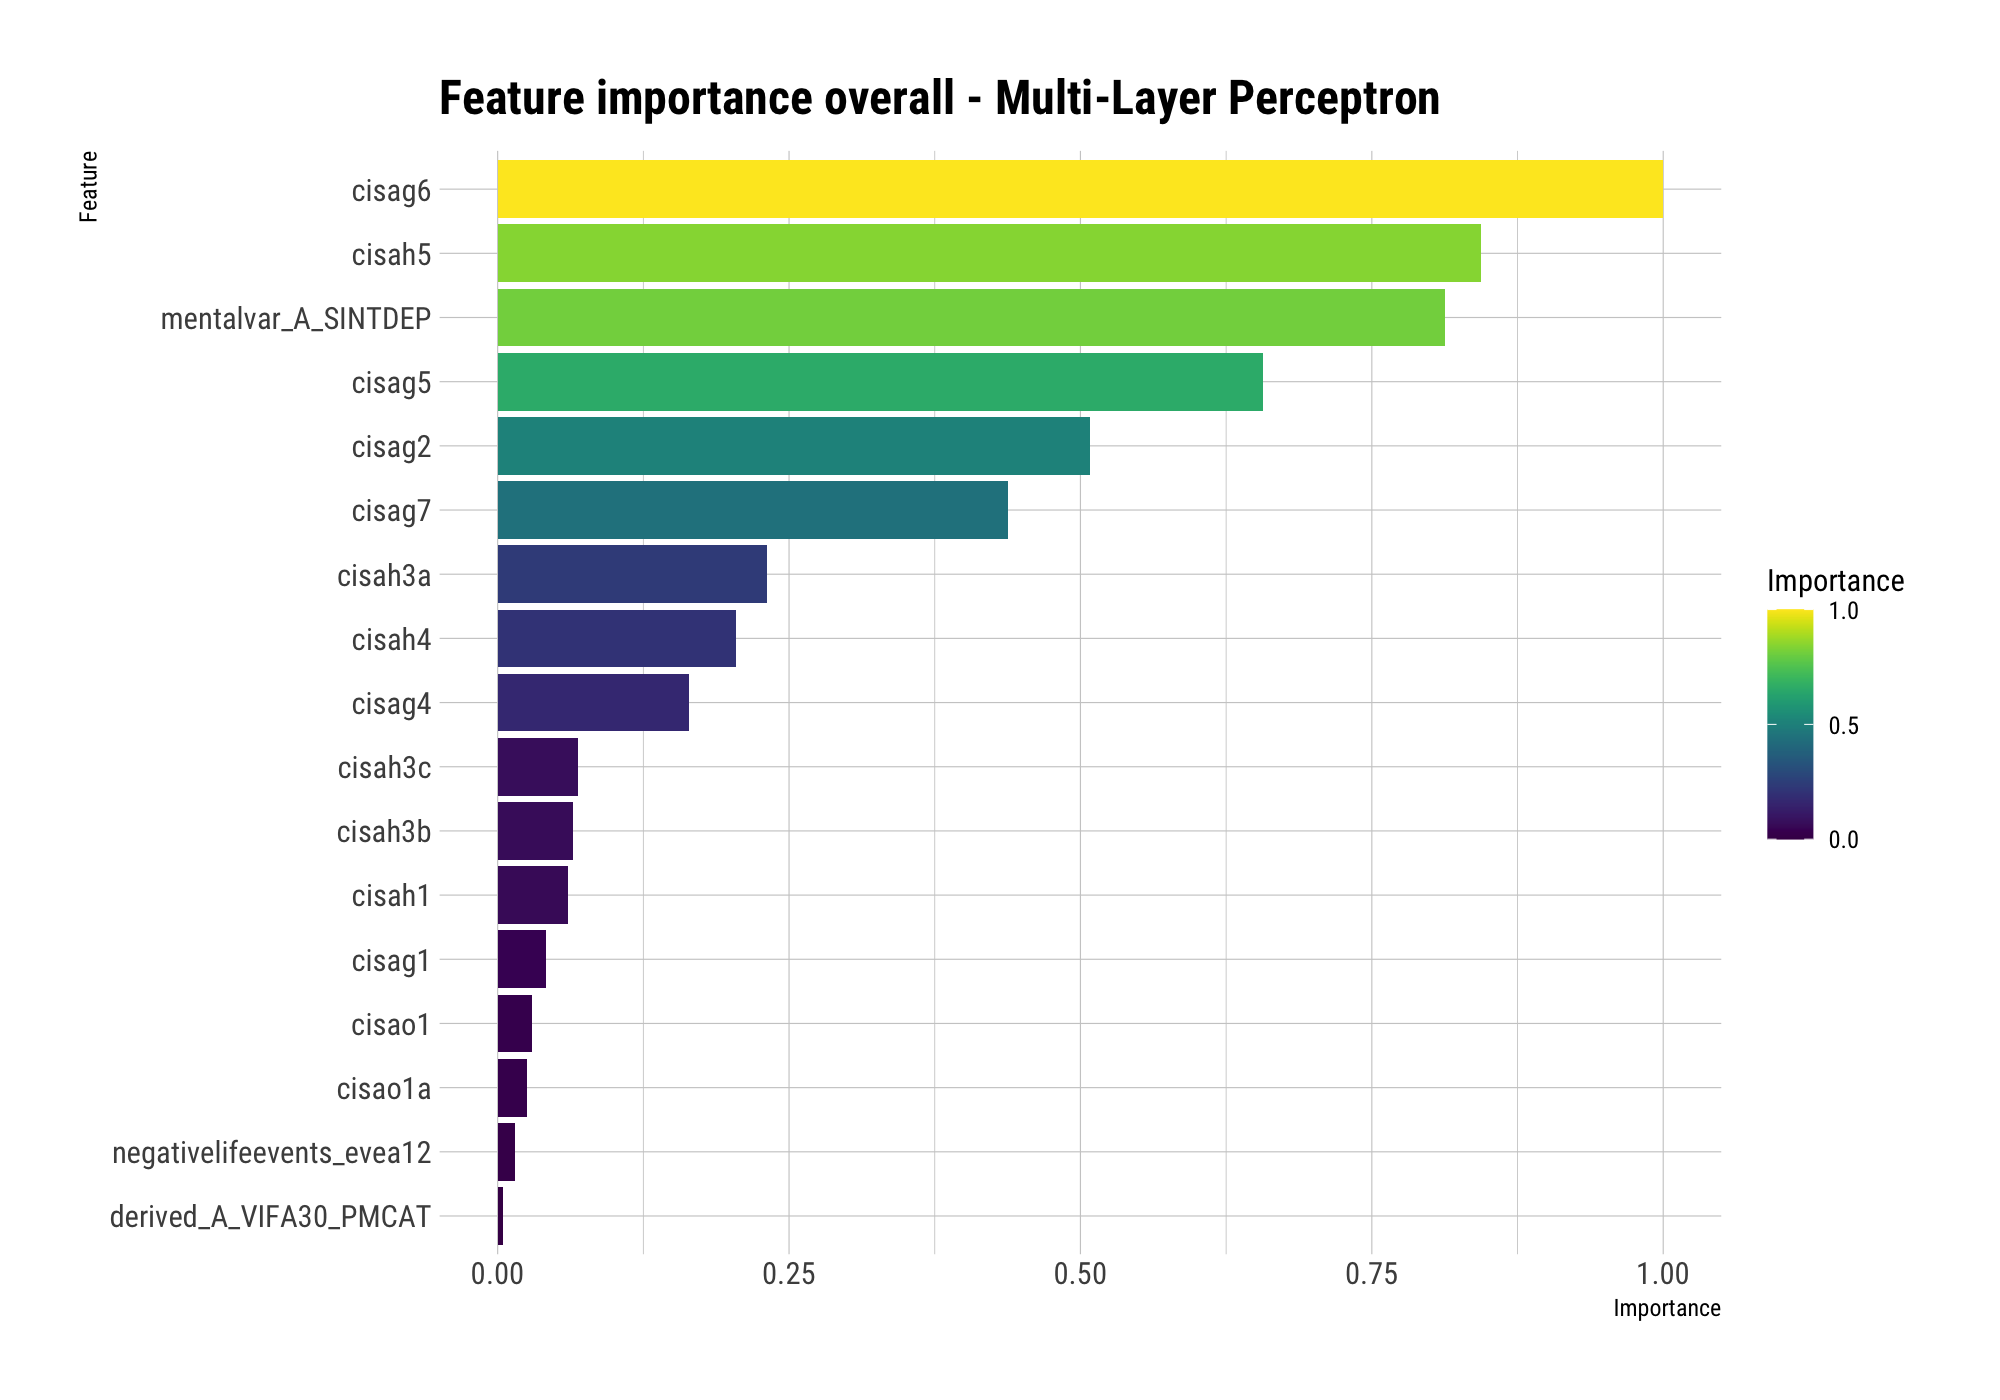
\includegraphics[scale=.16]{../../reports/results/models_and_evals/summary/var_imp_mlpML.png}}
            \label{fig:rank-mlp}
        \end{figure}
    }
    \frame{
        \frametitle{Rank de Atributos - Florestas Aleatórias}
        \begin{figure}[H]
            \centerline{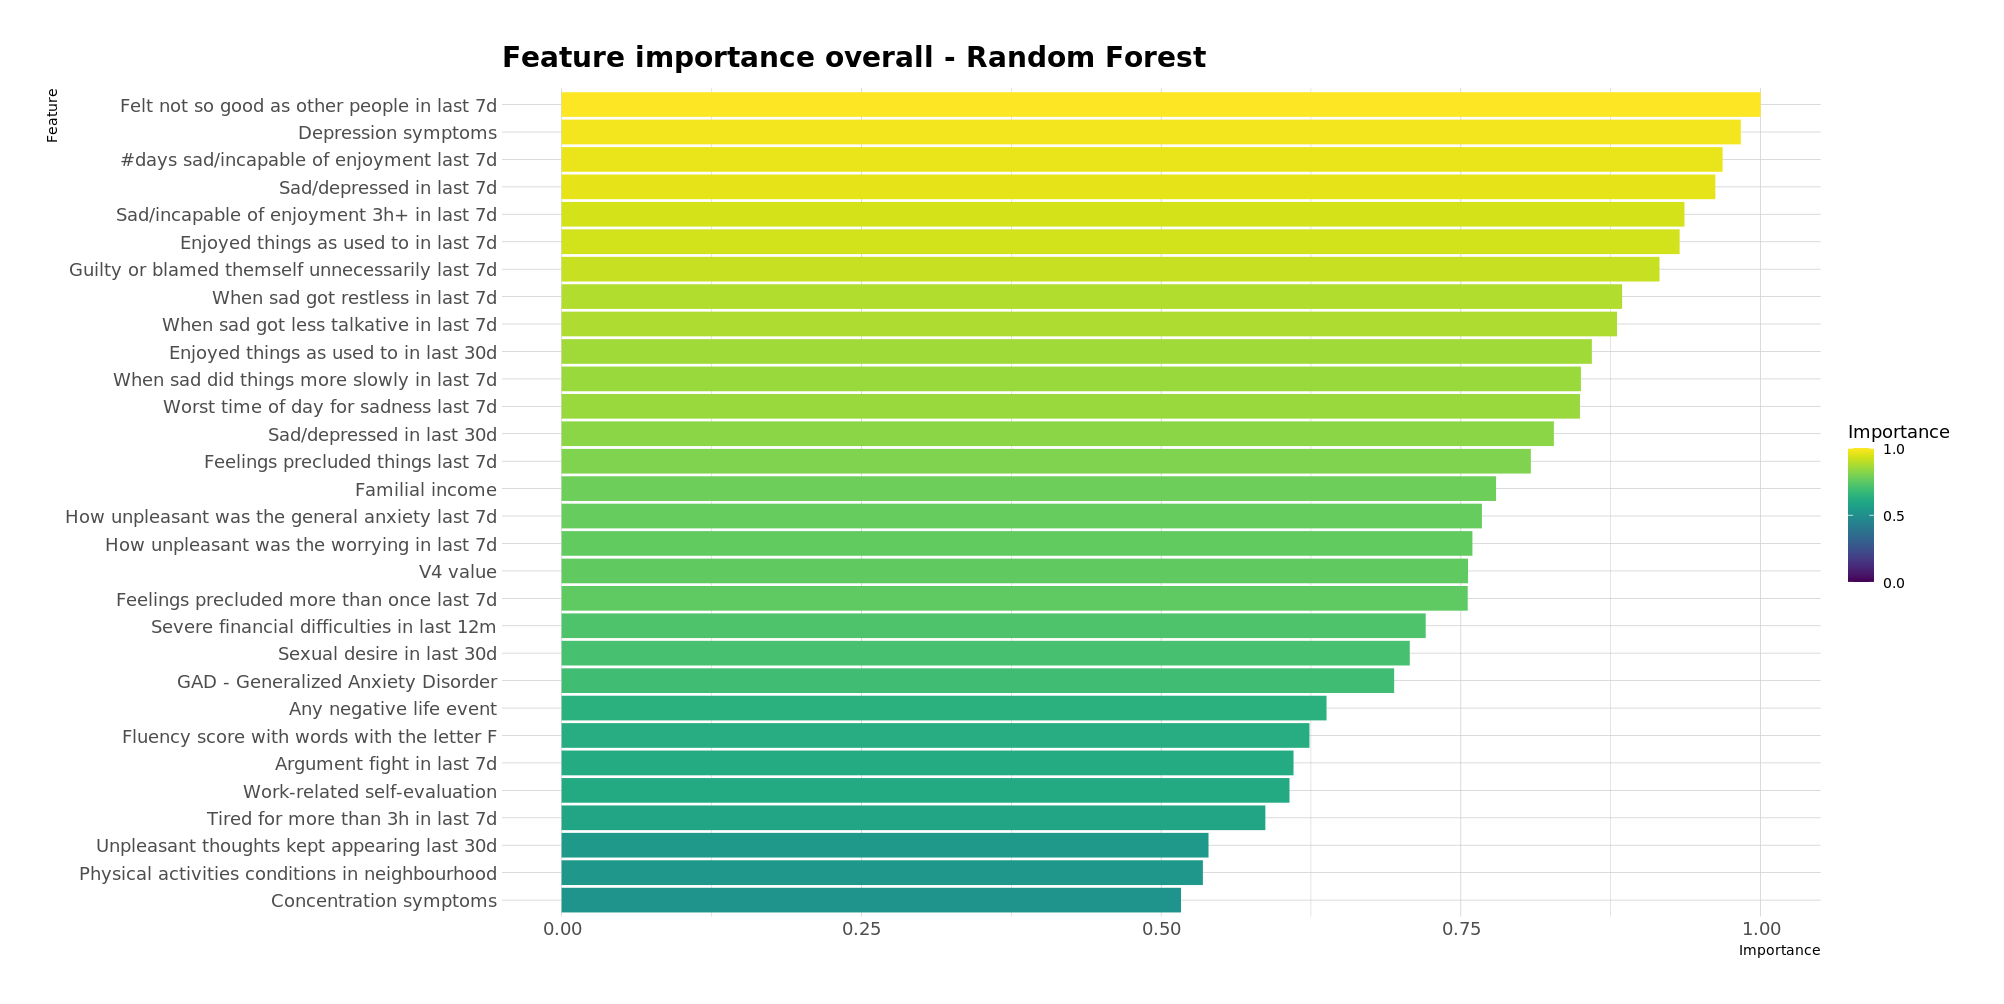
\includegraphics[scale=.16]{../../reports/results/models_and_evals/summary/var_imp_ranger.png}}
            \label{fig:rank-ranger}
        \end{figure}
    }
    \frame{
        \frametitle{Rank de Atributos - Ensemble}
        \begin{figure}[H]
            \centerline{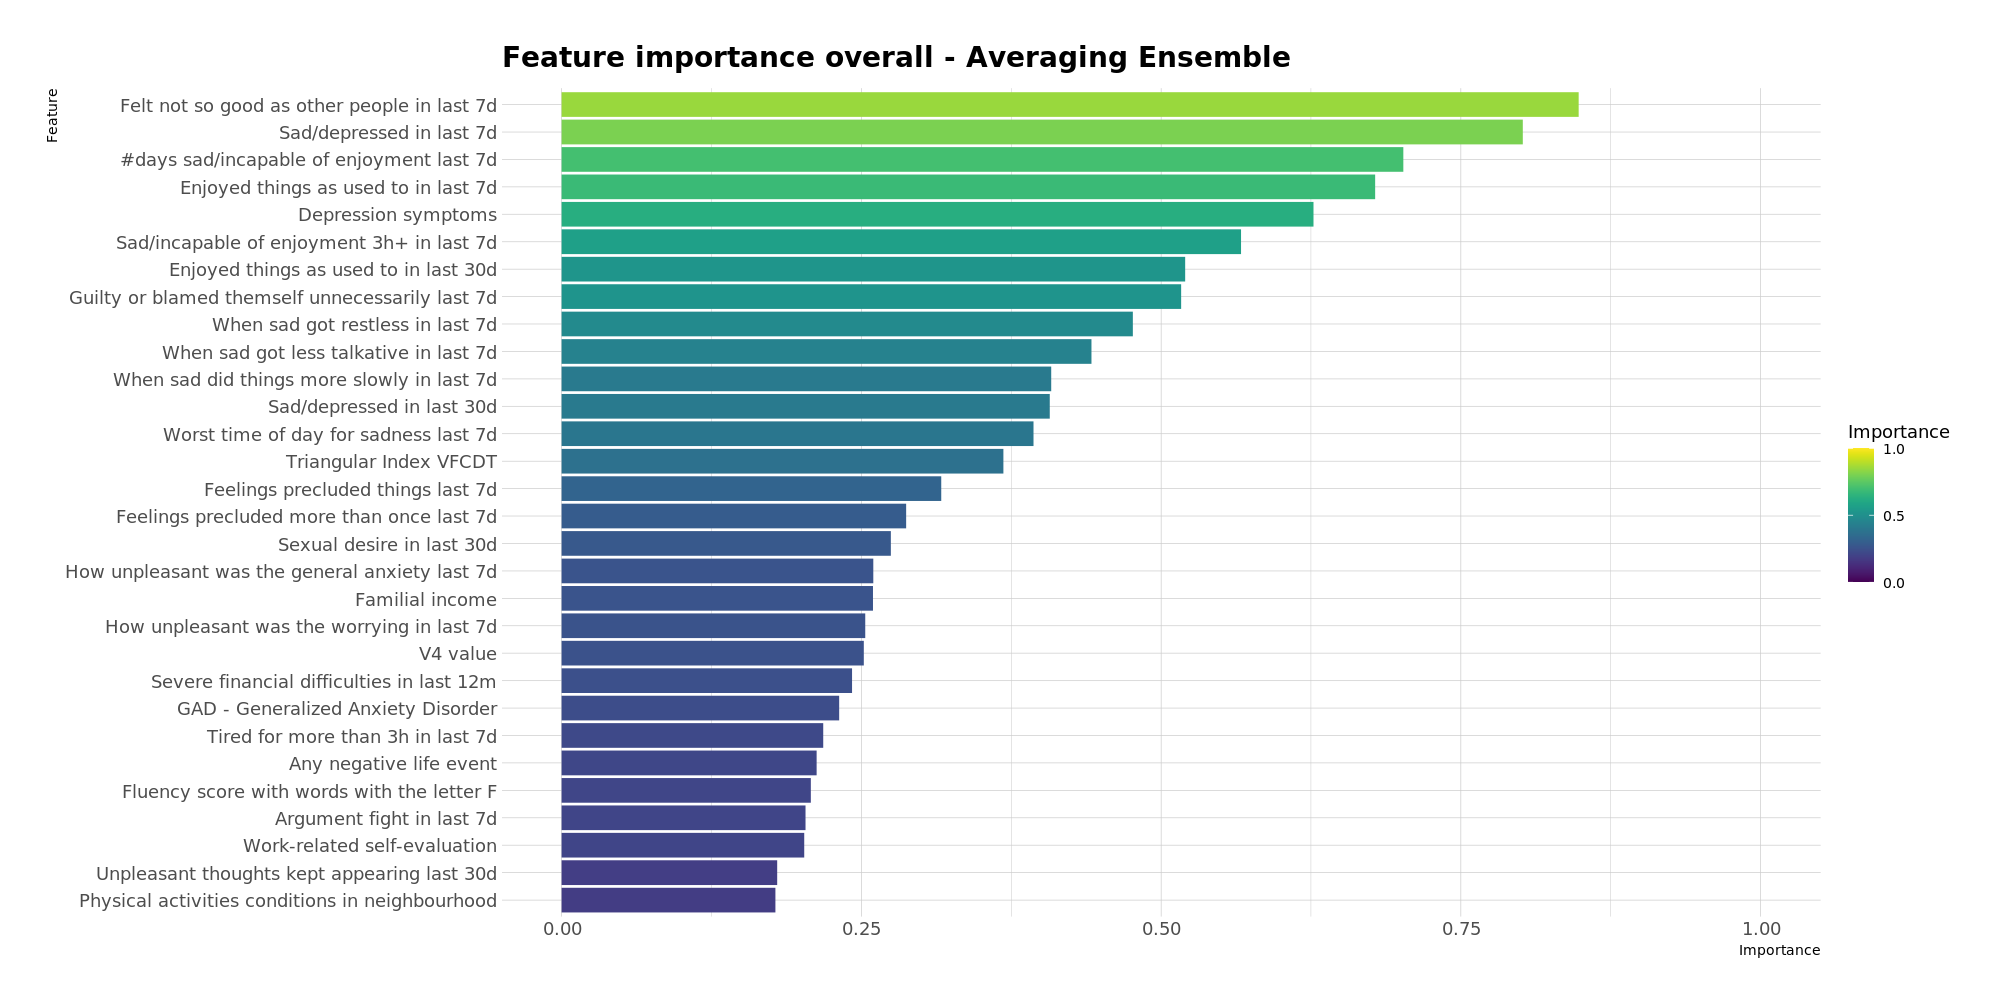
\includegraphics[scale=.16]{../../reports/results/models_and_evals/summary/var_imp_aggregation.png}}
            \label{fig:rank-ensemble}
        \end{figure}
    }
    \frame{
        \frametitle{Sumário de Atributos}
        \begin{enumerate}
            \item Sentimento de inferioridade
            \item Tristeza
            \item Desaparecimento de interesses
            \item Auto-culpa desnecessária
            \item Energia (disposição)
            \item Incapacidade de realizar atividades
            \item Renda
            \item Ansiedade
            \item Preocupação
            \item Libido
            \item Irritabilidade
            \item Obsessão
            \item Atividades físicas
        \end{enumerate}
    }


    \section{Conclusões}
    \begin{frame}[plain]
        \sectionpage
    \end{frame}

    \frame{
        \frametitle{Contribuições e Impacto}
        Classificação de suicidalidade com o ELSA-Brasil\linebreak\linebreak
        Relevância de variáveis para classificação\linebreak\linebreak
        Metodologia (desbalanço de classes, RFE, etc.)
    }
    \frame{
        \frametitle{Contribuições e Impacto}
        \begin{table}[h]
            \caption{Estimativas de desempenho - comparação com trabalhos similares}
            \begin{center}
                \begin{tabular}{c|c|c|c|c|c}
                    \textit{Paper} & \textit{Algorithm} & \textit{F\textsubscript{2}-Score} & \textit{AUCROC} & \textit{Sens.} & \textit{Espec.} \\
                    \hline
                    \hline
                    A              & XGB                & 0.84                              & 0.86            & 0.79           & 0.79            \\
                    B              & ANNs+RF            & 0.71                              & 0.88            & 0.80           & 0.79            \\
                    \textbf{Ours}  & \textbf{EN/ANN/RF} & \textbf{0.69}                     & \textbf{0.81}   & \textbf{0.78}  & \textbf{0.67}   \\
                    C              & ANN                & 0.48                              & 0.88            & 0.81           & 0.77            \\
                    D              & EN                 & 0.45                              & 0.79            & 0.67           & 0.78            \\
                    \hline
                \end{tabular}
            \end{center}
            \legend{

                A: JUNG et al. (2019);

                B: ROY et al. (2020);

                C: OH et al. (2020);

                D: LIBRENZA-GARCIA et al. (2020).}
            \label{tab:related-work-vs-ours}
        \end{table}

    }
    \frame{
        \frametitle{Possíveis Aprimoramentos}
        Análise de variação de valores dos atributos\linebreak\linebreak
        Explorar mais os dados do ELSA-Brasil\linebreak\linebreak
        Estudo com foco clínico\linebreak\linebreak
        Aplicações de assistência e suporte clínicos\linebreak\linebreak
    }

    \section*{}

    \begin{frame}
        \frametitle{Agredecimentos Especiais}
        André Russowsky Brunoni (USP) \linebreak\linebreak
        Ives Cavalcante Passos (UFRGS) \linebreak\linebreak
        Mariana Recamonde Mendoza (UFRGS)
    \end{frame}

    \begin{frame}
        \frametitle{Obrigado!}
        \InfContacts
    \end{frame}

\end{document}